\documentclass[11pt,a4paper,spanish]{mibook}
\usepackage[a4paper,left=3cm,right=2cm,top=3cm,bottom=2cm]{geometry}
\usepackage{graphicx}
\usepackage[T1]{fontenc}
\usepackage[utf8]{inputenc}
\usepackage[spanish]{babel}
\usepackage{natbib}
\usepackage{multirow}
\usepackage{url}
\usepackage{float}
\usepackage{amsmath}
\usepackage{amsthm}
\usepackage{amssymb}
\usepackage{mathtools}
\usepackage{multirow}
\usepackage{scalerel}
\usepackage[table,xcdraw]{xcolor}
\usepackage{longtable} % para tablas largas
\usepackage{enumerate}

%paquetes extras
\usepackage{subfigure}
\usepackage{amssymb}
\usepackage{algorithm}
\usepackage{algorithmic}
\usepackage{changepage}   % for the adjustwidth environment
\usepackage{tikz}
\usetikzlibrary{arrows}
\usetikzlibrary{trees}
\usetikzlibrary{automata}
\usetikzlibrary{positioning}
\usetikzlibrary{graphs}
\usetikzlibrary{calc}
\usetikzlibrary{arrows.meta}
\usetikzlibrary{shapes.geometric}
\usetikzlibrary{shapes.symbols}
\usepackage{url} 
\usepackage[colorlinks=true,linkcolor=black,citecolor = black, urlcolor = blue]{hyperref}
\usepackage{minted}
\usepackage{tabularx}
\usepackage{multicol}
\usepackage{multirow}
\usepackage{graphicx}
\usepackage{breakcites}
\usepackage{float}
\usepackage{stackrel}
\usepackage{color}
\usepackage[textsize=small, textwidth=2cm, spanish, colorinlistoftodos, 
backgroundcolor=blue!20, 
bordercolor=blue]{todonotes}
\floatname{algorithm}{Algoritmo}
\renewcommand{\algorithmicrequire}{\textbf{Entrada:}}
\renewcommand{\algorithmicensure}{\textbf{Salida:}}
\renewcommand{\algorithmicif}{\textbf{si}}
\renewcommand{\algorithmicthen}{\textbf{entonces}}
\renewcommand{\algorithmicelse}{\textbf{sino}}
\renewcommand{\algorithmicend}{\textbf{fin}}
\renewcommand{\algorithmicforall}{\textbf{para cada}}
\renewcommand{\algorithmicfor}{\textbf{para}}
\renewcommand{\algorithmicdo}{\textbf{hacer}}
\renewcommand{\algorithmicand}{\textbf{y}}
\renewcommand{\algorithmicor}{\textbf{o}}
\renewcommand{\algorithmicwhile}{\textbf{mientras}}
\definecolor{softred}{rgb}{1.0, 0.44, 0.37}
\usepackage{caption}
\DeclareCaptionFormat{algor}{%
	\hrulefill\par\offinterlineskip\vskip1pt%
	\textbf{#1#2}#3\offinterlineskip\hrulefill}
\DeclareCaptionStyle{algori}{singlelinecheck=off,format=algor,labelsep=space}
\captionsetup[algorithm]{style=algori}
\usepackage{mathtools}
\DeclarePairedDelimiter\ceil{\lceil}{\rceil}
\DeclarePairedDelimiter\floor{\lfloor}{\rfloor}
\newtheorem{definition}{{\bf Definición }}[section]
\newtheorem{ejemplo}{{\bf Ejemplo }}[section]
\newtheorem{theorem}{\bf Teorema}[section]
\newtheorem{property}{\bf Propiedad}[section]
%  Definición de Palabras Clave
\def\palabras{ 
	\mbox{{\boldmath $Palabras\;Clave$}{\bf: }}}
%\emph{Palabras Clave}
\def\endpalabras{\medskip\rm
}
\hyphenation{Co-ma-hue}
\hyphenation{Par-ti-cu-lar-men-te}
\hyphenation{me-ca-nis-mos}
\hyphenation{pro-ble-mas}
\hyphenation{in-te-rac-tuar re-pre-sen-ta-cion}
\hyphenation{do-mi-nios ra-zo-na-dor de-sa-rro-lla}



\begin{document}

\renewcommand{\tablename}{Tabla}
\renewcommand{\listtablename}{Indice de tablas}

%Empieza la numeracion en números romanos
\frontmatter
% Incluimos la cartula
%Observación: Si bien la página del prefacio dice que sea empty, debería comenzar alli la numeración. Se sugiere numeración romana. Recomenzar la numeración en el primer capítulo de la tesis  con numeración arábiga.

\titlepage

\begin{center}
\ \\
\ \\
\vspace{-1cm}
 

\ \\

\vspace{0.5cm}
{\Large{\bf \sc Universidad Nacional del Comahue}}\\

\ \\
{\Large { \sc Facultad de Informática}}\\

\vspace{-2.5cm}
\mbox{\hspace{-1cm}
\includegraphics[width=2.5cm,height=2.5cm]{imagenes/unc.png}\hspace{13cm} 
\includegraphics[width=2.5cm,height=2.5cm]{imagenes/fai.png}}


\vspace{6cm}

{\Large {\bf\sc Tesis de Licenciatura en Ciencias de la Computaci\'on}}\\
\ \\
\ \\
{\LARGE {\bf Layout Automático de Grafos con  Inteligencia Artificial para la Visualización de Modelos Conceptuales \\
}}\ \\
\vspace{3cm}



{\Large Giuliano Marinelli}\\
\vspace{2cm}

{\Large Laura Cecchi}\\

{\Large Germán Braun}\\
\ \\



\vfill
{\Large {\sc Neuqu\'en}\hspace{6cm}{\sc Argentina}}\\
\ \\

{\Large Marzo 2020}\\

\end{center}

\pagebreak





% Incluimos la pgina de prefacio.
\ \\
\ \\
\label{pagpref}
\noindent{\LARGE \sc Prefacio}\\
\ \\
\ \\
\ \\
\ \\
\ \\

Esta tesis es presentada como parte de los requisitos finales para optar al grado académico de {\em Licenciado en Ciencias de la Computación}, otorgado por la Universidad Nacional del Comahue, y no ha sido presentada previamente para la obtención de otro título en esta Universidad u otras. La misma es el resultado de la investigación llevada a cabo en el \emph{Departamento de Teoría de la Computación}, de la Facultad de Informática, en el período comprendido entre Octubre 2019 y Marzo 2020, bajo la dirección de la \emph{Dra. Laura Cecchi} y la codireccion del \emph{Dr. Germán Braun}.



\vspace{3cm}


\ \\
{\flushright Marinelli, Giuliano \\
{\sc Facultad de Informática \\
Universidad Nacional del Comahue}\\
{\em Neuqu\'en, 05 de Marzo de 2020}\\}

\vfill

\begin{center}
%
\framebox{\begin{minipage}[t]{0.9\columnwidth}%
\begin{flushleft}

\includegraphics[scale=0.035]{imagenes/unc.png}

\vspace{-2cm}
{\large \hspace{5cm}\sc universidad
nacional del comahue} \\
\par\end{flushleft}
\begin{center}
{\large \qquad{}}{ \hspace{2.5cm} Facultad de Informática}
\par\end{center}

\vspace{1cm}

\indent \ \ \ \ \ \ \ \ \ \ \ La presente tesis ha sido aprobada el día ........................., mereciendo la \\
\indent \ \ \ \  \ \ \ \ \ calificación de .............................

\medskip{}

\vspace{1cm}
\end{minipage}}
\end{center}

\pagebreak


% Incluimos la pgina de dedicatorias. Esta pgina es opcional.
% Si la pgina no quiere ser incluida anteponga el smbolo "%" al comienzo de la siguiente lnea
%%\ \\
\ \\
\label{pagdedic}
\noindent{\LARGE \sc Dedicatorias}\\
\ \\
\ \\

\ \\

\ \\
\ \\


\vfill
\pagebreak



% Incluimos la pgina de agradecimientos. Esta pgina es opcional.
% Si la pgina no quiere ser incluida anteponga el smbolo "%" al comienzo de la siguiente lnea
%%\ \\
\ \\
\label{pagagrad}
\noindent{\LARGE \sc Agradecimientos}\\
\ \\
\ \\

\ \\

\ \\
\ \\


\vfill
\pagebreak


% Incluimos la pgina de resumen
\ \\
\ \\
\label{pagresum}
\noindent{\LARGE \sc Resumen}\\
\ \\
\ \\

\ \\

\ \\
\ \\


\vfill
\pagebreak


% Incluimos la pgina de resumen en ingls
\ \\
\ \\
\label{pagsumm}
\noindent{\LARGE \sc Abstract}\\
\ \\
\ \\

\ \\

\ \\
\ \\
The automatic layout algorithms are great utility tool for the design of conceptual models, diagrams or graphs, in any modeling language like UML, ER, ORM, among others. In this sense, for achieve a layout algorithm is necessary the study of several features of that conform a correct visualized layout. We have considered of great importance, among others features, that the graph (or diagram) resulting must have a minimum crossing number between their edges. This problem is known as Crossing Number, and is NP-Complete. 

In this work we introduce the design and the implementation of {\sc ArcGen}, a new genetic algorithm, that minimize the crossing number of a graph. {\sc ArcGen} involves a preprocessing of the original graph, that transforms the graphic representation into an Arc Diagram or Linear Embedding. We described all the details of the design and the implementation of the algorithm. 

Finally, giving the motivation of the development of {\sc ArcGen} and the temporal complexity of the Crossing Number problem, some experiments are made, circumscribed to a graph with a proportional size to the diagrams generated in real practice conceptual modeling. 

We present the results of this experiments, showing that the algorithm reduces the crossing number of the original graph in up to four times. We also show the integration of the mentioned algorithm with other layout algorithms like the Force Directed Layout Algorithm by Tunkelang which allows to give a different visualization of the graph, and are evaluated and compared the overall results and by separated.

\vfill
\pagebreak


% Tabla de contenido o Indice del contenido
\tableofcontents{}

% Lista de figuras o Indice de figuras
\listoffigures

% Lista de tablas o Indice de Tablas
\listoftables

%Empieza la numeracin en nmeros arbigos
\mainmatter
\chapter{Introducci\'on}\label{cap1}

\section{Motivaci\'on}
Actualmente, las herramientas de  modelado gráficas  y automáticas que asisten a los  modeladores son esenciales  debido al incremento  en la complejidad de los sistemas de información. Una mala disposición gráfica de los elementos del  diagrama en el modelo hace que sea difícil de leerlo y de comprenderlo en forma inmediata \cite{Sto14,Sto11,Huang07,ware02}.
	
	Los algoritmos de layout automáticos permiten el reordenamiento de los  elementos gráficos de los diagramas de modelado, de manera que se disponga una visualización más satisfactoria de los mismos, como puede verse en la Figura \ref{fig:ejemplo_crossnum}.
	Sin embargo, por estar basados en problemas de optimización combinatorios, heredan la  complejidad computacional de éstos,  que en su mayoría  son  NP-Completos \cite{Papadimitriou1976, Garey:1974}. 
	
	\begin{figure}[h]
		\centering
		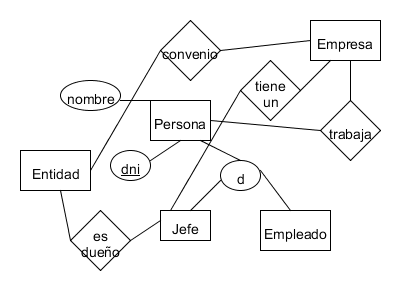
\includegraphics[width=5cm]{imagenes/ejemplo_malo.png}
		\hspace{1.5cm}
		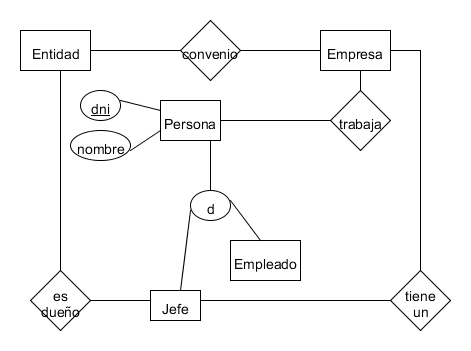
\includegraphics[width=5cm]{imagenes/ejemplo_bueno.png}
		\caption{Dos formas de dibujar un diagrama ER. El primer diagrama presenta 3 cruces, y no resuelve una disposición geométrica de los elementos, en cambio el segundo mejora estos aspectos.}
		\label{fig:ejemplo_crossnum}
	\end{figure}
	
	
	
	%	 A good drawinq is one in which no two arcs incident with a common node have a common point, and no two arcs have more than one point in common.
	
	%Para este trabajo se plantea un algoritmo que recibirá como entrada un modelo conceptual expresado en diferentes lenguajes como UML, ER, ORM, etc, y se buscará un
	
	En este trabajo se introduce un nuevo algoritmo  genético,  denominado \textsc{ArcGen},  que es el  punto de partida  para  resolver el problema de la correcta visualización de un modelo conceptual expresado en UML o  ER  y que busca ser incorporado a {\it Crowd} \cite{gimenez2016crowd}. {\it Crowd} es una herramienta web para modelado ontológico utilizando los lenguajes  UML \cite{booch2005unified}\ y  ER \cite{chen1988entity}, con soporte de razonamiento para asistir al usuario en tareas de diseño y validación. 
	
	Nos centramos en la resolución del problema de Crossing Number, motivados por la  importancia  estética de reducir el número de cruces de arcos en la representación gráfica de grafos \cite{Kob14}. Este es un problema NP-Completo \cite{garey1983crossing} de gran importancia para la visualización de grafos, que radica en evitar, en la mayor medida posible, que los arcos de un grafo dibujado sobre el plano Euclídeo se crucen.
	%de manera que se obtenga un grafo con menos puntos de  cruces de arcos  respecto del grafo original. 
	Asimismo, circunscribimos la solución que se propone  a grafos con ciertas características encontradas en los diagramas de modelado conceptual (tamaño y complejidad).
	
	% de grafos de entrada, es decir, que obtendrá un resultado eficiente considerando parámetros normales de entrada.
	
	El algoritmo \textsc{ArcGen} involucra un preprocesamiento del grafo original,  transformando su representación a una  forma particular, llamada Diagrama de Arcos \cite{saaty1964minimum} o Linear Embedding \cite{masuda1990crossing} según las diferentes fuentes. Un Diagrama de Arcos \cite{Wat02,Nich68,saaty1964minimum}\ es una representación de  un grafo en un plano, donde los nodos se ubican sobre una recta, como puede visualizarse en la Figura \ref{fig:arcdiagram_k6_no_optimo}. Esta representación del grafo tiene la cualidad de %no generar cruces de arcos provocados por la representación, si no, 
	que los cruces obtenidos dependerán del ordenamiento de los nodos, esto es, su disposición sobre la línea y del  semiplano en el que se  dibuja el arco, es decir, como un semicírculo por arriba de la recta o por debajo de ella. %Por lo tanto, esta representación nos facilita el desarrollo de un algoritmo para la resolución parcial de Crossing Number.
	Inicialmente, se trabajó sobre grafos completos \cite{Aich02}, buscando un ordenamiento de sus nodos que generen un número mínimo de cruces de arcos.
	%Dada esta forma gráfica de un grafo, se propone en un principio buscar un ordenamiento para permitir que grafos completos (aquellos en que cada par de nodos está conectado por un arco) dispongan de un número de cruces de arcos mínimo.
	Este problema se ha podido solucionar satisfactoriamente con un algoritmo simple, permitiendo cumplir con la cota superior dada por la conjetura de Guy \cite{guy1960combinatorial}. %, como se verá en la sección \ref{sec:arcdiagram}.
	Sin embargo,  al utilizar este algoritmo sobre grafos no completos, las  mejoras obtenidas en el número de cruces no fueron suficientes, lo que dió génesis a {\sc ArcGen}.
	
	La  población inicial de {\sc ArcGen}  está generada a partir de la representación Diagrama de Arcos mejorada del  grafo original, lo que guía la búsqueda del menor número de cruces.%, explicado en la sección \ref{sec:genetico}.
	
	Los resultados experimentales realizados sobre grafos no dirigidos de tamaño moderado muestran que  {\sc ArcGen} se comporta en forma satisfactoria, disminuyendo en algunos casos hasta en 4 veces la cantidad de cruces sobre la representación original. 
	%\todo[inline, color=green]{Creo que habria que agregar un párrafo  de otras herramientas que analizaste y marcar diferencias. Diferencia con otros es que la  población inicial del  algoritmo genético parte de un grafo preprocesado.}
	
	Existen otros  algoritmos genéticos que resuelven el problema, como  TimGA \cite{eloranta2001timga}\ el cual, a diferencia del algoritmo \textsc{ArcGen}, propuesto en este trabajo, utiliza grafos genéricos para la representación de sus individuos, almacenando las posiciones $x$ e $y$ de cada nodo en matrices y considerando la representación gráfica de los arcos como rectas entre tales nodos. Esta representación produce gran cantidad de variaciones y posibles grafos, haciendo que el algoritmo genético deba realizar mayor cantidad de generaciones, además de no permitir la representación de arcos curvos. De esta manera, genera implícitamente mayor cantidad de cruzamientos. 
	
	Por otro lado, el propuesto por Hongmei He et al. \cite{he2007parallelisation}\ considera la representación  Diagrama de Arcos, pero comienza con una población generada aleatoriamente a diferencia de \textsc{ArcGen} que genera la población a partir de un individuo dado por el algoritmo de grafos completos. Esto causa que el algoritmo consuma más tiempo en alcanzar un máximo local o global, quitándole practicidad para el objetivo buscado.
	
	En el survey de Helen Gibson et al. \cite{gibson2013survey} se han recopilado gran variedad de algoritmos de layout, de los cuáles el más adecuado, con respecto a precisión y velocidad, para layout en modelado conceptual, es el algoritmo Dirigido por Fuerzas de Tunkelang \cite{tunkelang1998jiggle}. Este algoritmo  propone un modelo físico donde los nodos y arcos realizan fuerzas de repulsión entre ellos para evitar cruzamientos. Esta simulación se realiza por un tiempo dado hasta obtener el resultado deseado. Tal algoritmo puede variar la eficacia del resultado según las posiciones iniciales del grafo de entrada y sobre grafos con mucha densidad es menos efectivo, por lo que los algoritmos de este trabajo buscan mejorar este aspecto. %, por lo que se consideró abordar el problema desde un modelo jerárquico, el cual consta de un reordenamiento de posiciones fijas, tal como se realiza en los algoritmos genéticos mencionados anteriormente.
	
	%Este trabajo está organizado de la siguiente manera. En la sección \ref{sec:arcdiagram},  se propone un algoritmo  que esquematiza  un grafo arbitrario en un Diagrama de Arcos optimizado para grafos completos. En la sección \ref{sec:genetico}, se explica el algoritmo genético desarrollado para minimizar la cantidad de cruces de arcos  respecto del  grafo original. Luego en la sección \ref{sec:implementacion}, se describe la aplicación que genera el grafo optimizado. En la sección \ref{sec:resultados}, se presentan resultados experimentales realizados  sobre la aplicación. Finalmente, se presentan las conclusiones y trabajos futuros.

\section{Objetivos y Contribuciones}
El objetivo general de este trabajo es el diseño e implementación  de un algoritmo de layout automático de grafos para la visualización en herramientas de modelado conceptual. Se pretende trabajar en un diseño que utilice técnicas de Inteligencia Artificial y que  permita adaptar las funcionalidades de visualización de los diagramas, considerando los diferentes lenguajes de modelado conceptual, como EER, UML y \mbox{ORM 2.}
Se espera que los expertos o modeladores puedan utilizar tales herramientas de acuerdo a sus preferencias de notación con una disposición apropiada de los elementos visuales de los lenguajes de modelado conceptual, lo que redituará en una mejor legibilidad y un adecuado entendimiento del diagrama, potenciando la comunicación entre los interesados en la información del modelo.

Las principales contribuciones de este trabajo son:

\begin{itemize}
\item Diseño e implementación de un algoritmo que permite resolver un mínimo crossing number sobre diagramas de arcos para grafos completos.

\item Diseño e implementación de un algoritmo que permite alcanzar un mejor crossing number sobre  grafos no completos utilizando técnicas de algoritmos genéticos.

\item Integración de los algoritmos desarrollados con otros algoritmos de layout como el dirigido por fuerzas de Tunkelang.

\item Implementación de una herramienta de prueba para los algoritmos desarrollados.

\end{itemize}

\section{Estructura de la Tesis}
La tesis incluye los contenidos necesarios para que su lectura sea auto contenida, asumiéndose conocimientos a nivel de grado de teoría de la computación, programación y complejidad computacional. A continuación se describe la estructura de esta Tesis.

\subsubsection{Capítulo 1: Introducción}
En este capítulo se presenta la motivación, los objetivos, contribuciones y la organización de esta Tesis

\subsubsection{Capítulo 2: Antecedentes Conceptuales}
Se describen los conceptos teóricos fundamentales para este trabajo. Se describen algunos conceptos de teoría de grafos, problemas NP, algoritmos de layout y algoritmos evolutivos y genéticos.

\subsubsection{Capítulo 3: Diseño de los Algoritmos Propuestos}
Se describe el diseño de los algoritmos desarrollados, como interactúan entre ellos y su integración con otros posibles algoritmos.

\subsubsection{Capítulo 4: Implementación de los Algoritmos Propuestos}
Se describe la herramienta implementada para la depuración de los algoritmos, las especificaciones técnicas de la misma, y la integración con otra librería que provee el algoritmo de layout dirigido por fuerzas.

\subsubsection{Capítulo 5: Resultados Experimentales}
Se muestran los resultados obtenidos a partir de la ejecución de conjuntos de pruebas para medir la eficiencia de los algoritmos de este trabajo.

\subsubsection{Capítulo 6: Trabajos Relacionados}
Se exponen los diferentes trabajos que fueron relevados. Se los compara entre ellos y se analiza su efectividad para ser aplicados en el campo de modelado conceptual.

\subsubsection{Capítulo 7: Conclusiones}
 Finalmente, se presentan las conclusiones de esta tesis, los resultados obtenidos, avalados con publicaciones en congresos con referato y se proponen algunas ideas para trabajos futuros.

% La tesis incluye los contenidos necesarios para que su lectura sea auto contenida, asumiéndose
% conocimientos a nivel de grado de lógica clásica, representación de conocimiento y ontologías, y
% arquitecturas de software. A continuación se describe la estructura de esta Tesis.
% Capítulo 1: Introducción
% En este capítulo se presenta la motivación, los objetivos, contribuciones y la organización
% de esta Tesis.
% Capítulo 2: Variabilidad en SPL
% Se describen los modelos de variabilidad ortogonal detallando cada uno de los elementos
% e interacciones que los conforman. Posteriormente, se explica el proceso de análisis de
% variabilidad automático de los diagramas OVM, enfocándose principalmente en la detección
% de problemas.
% Capítulo 3: Técnica de Análisis Automatizado para OVM
% Se describe la técnica utilizada para realizar el análisis de variabilidad automatizado. Se
% introducen las Lógicas Descriptivas y se detalla la codificación en ALCI de los modelos
% OVM. Por último, se describen los principales antipatrones a identificar durante el proceso
% de Detección de Problemas.
% Capítulo 4: Diseño de la Herramienta
% En este capítulo, se describe el proceso de detección de problemas y posteriormente, se
% detalla el modelo cliente-servidor propuesto, los módulos y los diseños preliminares que
% cumplen con los objetivos propuestos por esta tesis.
% Capítulo 5: Implementación de la Herramienta
% Se describe a crowd-variability, una implementación de la herramienta. Se detallan los
% cambios realizados gráficamente al diseñar las primitivas, la representación intermedia de
% los modelos y el editor gráfico, entre otros. Se concluye el capítulo con un ejemplo de uso
% de la implementación, donde se muestra su funcionamiento con un modelo que no presenta
% antipatrones y otro que presenta.
% Capítulo 6: Trabajos Relacionadas
% Se introducen una serie de enfoques relacionados que fueron relevados. Se los compara con
% crowd-variability, considerando el lenguaje de modelado de variabilidad, el uso de lenguajes
% gráficos para el modelado, el método de formalización de los diagramas y la utilización de
% servicios de razonamiento subyacentes.
% Capítulo 7: Conclusiones
% Finalmente, se presentan las conclusiones de esta tesis, los resultados obtenidos, avalados
\chapter{Antecedentes Conceptuales}\label{cap2}

\section{Teoría de Grafos}
\label{sec:teoria_grafos}
La teoría de grafos es un rama que estudia las propiedades de los grafos. Concibe formalismos para representarlos de manera matemática, como también de forma gráfica. Un grafo $G=(V,E,\psi)$ está definido por un conjunto de vértices o nodos $V$, un conjunto de aristas o arcos $E$ y una función $\psi$ que asocia cada arista en $E$ con un par no ordenado de vértices en $V$ \cite{bondy1976graph}\cite{dubinsky1984mathematical}.

Los grafos pueden ser representados gráficamente a partir del dibujado sobre un plano de sus vértices como puntos y sus aristas como líneas que conectan tales puntos. 

\subsection{Estilos de Dibujado de Grafos}
\label{sec:estilos_de_dibujado}
 Para poder dibujar un grafo se debe, mínimamente, posicionar cada vértice sobre un punto $(x,y)$ sobre el plano, y luego unirlos mediante líneas según correspondan sus aristas. Dependiendo del estilo que se utilice los aristas pueden dibujarse como líneas rectas, curvas o por cadenas poligonales (líneas articuladas) \cite{nishizeki2004planar}.
 
\subsubsection{Dibujado Planar}
Un dibujado planar de un grafo es aquel en la que no hay intersección entre ningún par de aristas. Es posible dibujar un grafo de manera planar o no planar, pero no todos los grafos tienen un dibujado planar. Un grafo que admite al menos un dibujado planar es llamado grafo planar.

\begin{figure*}[h]
	\centering
	\subfigure[Grafo dibujado de manera planar]{
		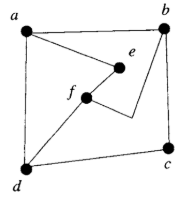
\includegraphics[width=0.33\textwidth]{imagenes/grafo_planar_1.png}
		\label{subfig:ejemplo_dibujado_planar}
	}
	\subfigure[El mismo grafo dibujado de manera no planar]{
		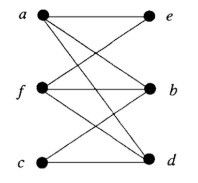
\includegraphics[width=0.33\textwidth]{imagenes/grafo_no_planar_1.png}
		\label{subfig:ejemplo_dibujado_no_planar}
	}
	\caption{Ejemplo de grafo planar. Dibujado de manera planar y no planar \cite{nishizeki2004planar}.}
	\label{fig:ejemplo_dibujado_planar}
\end{figure*}

\subsubsection{Dibujado Diagrama de Arcos}
\label{sec:dibujado_diagrama_de_arcos}

Un Diagrama de Arcos \cite{Wat02} es un estilo con el  que se dibuja un grafo, en el que los vértices del grafo se ubican sobre  una línea en el plano  Euclídeo y los arcos se dibujan como  semicírculos sobre alguno de los dos  semiplanos delimitados por la línea o bien pueden ser segmentos de la línea, siempre que conecten vértices que son consecutivos en la recta.
En la Figura \ref{fig:arcdiagram_ejemplo} se muestra un ejemplo con 6 nodos.

\begin{figure}[h]
	\centering
	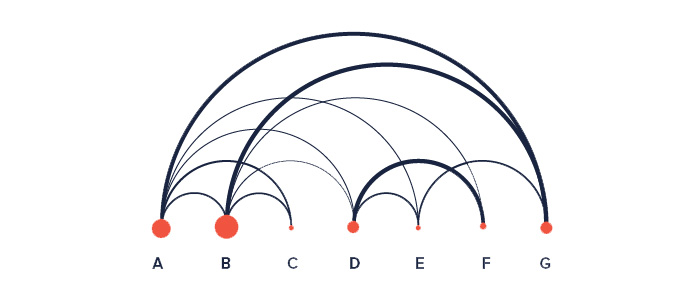
\includegraphics[width=12cm]{imagenes/diagrama-de-arco.jpg}
	\caption{Ejemplo de un diagrama de arcos.}
	\label{fig:arcdiagram_ejemplo}
\end{figure}

%imagen de grafo arc diagram

\subsection{Propiedades de Dibujado de Grafos}
\label{sec:propiedades_dibujado_grafos}
Los grafos pueden dibujarse de infinitas formas, pero al momento de dibujar un grafo para un uso específico se consideran una variedad de propiedades que brindan medidas para fortalecer ciertas características que quieran destacarse o mejorarse de un dibujo para así hacerla mas intuitiva según su dominio.\\

\begin{property}[Área]
	Es el área que ocupa el plano donde se dibuja el grafo. Si el área es de gran tamaño, produce que tengamos que visualizarlo mediante muchas páginas o desplazarnos sobre el plano. En cambio, si disminuimos la resolución se vuelve mas dificultoso de leer. En este sentido, se busca una relación de aspecto favorable entre el tamaño y la resolución.
\end{property}

\begin{property}[Cruces de Arcos]
	Los cruces o intersecciones de arcos abren a posibles confusiones de lectura, por lo que en cualquier dibujado siempre se busca disminuir lo mas posibles la cantidad de cruces.
\end{property}

\subsection{Aplicaciones de grafos}
Pueden utilizarse los grafos para diversas aplicaciones. Una de principal interés es la visualización de modelos conceptuales, permitiendo representarlos ante una notación particular de cada tipo de modelado.

%imagenes de modelos conceptuales (uml, er, orm)

\section{Problemas NP}
\label{sec:problemas_np}
Los problemas NP son aquellos que se encuentran categorizados en la clase de complejidad temporal NP (\emph{nondeterministic polynomial  time}). La clase NP abarca un conjunto de problemas de decisión los cuales pueden ser resueltos en un tiempo polinomial por una Máquina de Turing No Determinística, a partir de ahora MTND \cite{arora2009computational}.

Formalmente en términos de $\text{NTIME}$ se define como:

$$\text{NP} = \bigcup_{k \in  \mathbb{N}}^{}{\text{NTIME}(n^k)}$$

donde $\text{NTIME}(n^k)$ es el conjunto de problemas que pueden resolverse por una MTND en tiempo $O(n^k)$.

Entre estos problemas se considera de interes el problema de Crossing Number.

\subsection{Crossing Number}
\label{sec:crossing_number}
Una de las propiedades fundamentales de dibujado de grafos \ref{sec:propiedades_dibujado_grafos} es el número de cruces de arcos, \emph{crossing number} a partir de ahora, o $v(G)$ de un grafo $G=(V,E)$. Esta es, el menor número entero $K$ tal que $G$ puede ser dibujado en el plano, donde no haya mas de $K$ intersecciones entre los arcos graficados del conjunto $E$.

En general, el problema de decisión de \emph{crossing number} se define como ``Dado un grafo $G$ y un número entero $K$, ¿es $v(G) \leq K$?"

Este problema es considerado dentro de la clase de complejidad NP \cite{garey1983crossing}.

\section{Algoritmos de Layout de Grafos}
Los algoritmos de layout de grafos responden a una clase particular de problemas de optimización combinatorios, cuyo objetivo es encontrar un layout lineal de un grafo de entrada de manera que una determinada función sea optimizada. Un layout lineal es un etiquetado de los nodos de un grafo con un número entero distintivo \cite{diaz2002survey}, como se muestra en la figura \ref{fig:ejemplo_grafo_linear}.

\begin{figure*}[h]
	\centering
	\subfigure[Grafo etiquetado con un layout lineal.]{
		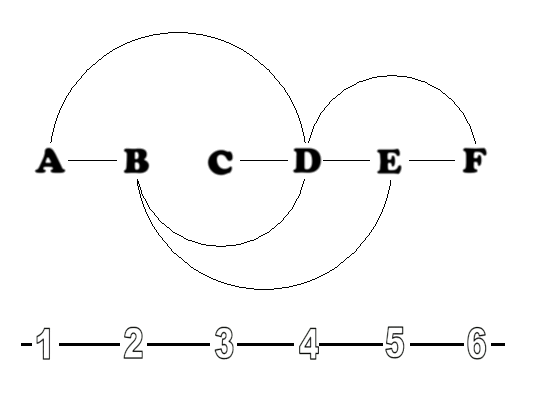
\includegraphics[width=0.39\textwidth]{imagenes/grafo_linear_2.png}
		\label{subfig:ejemplo_grafo_linear_original}
	}
	\subfigure[El mismo grafo etiquetado con otro layout lineal.]{
		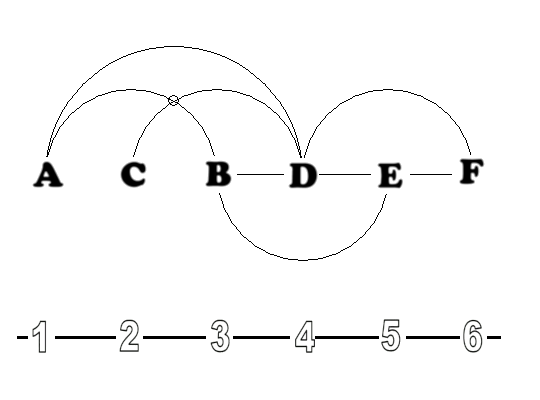
\includegraphics[width=0.39\textwidth]{imagenes/grafo_linear_1.png}
		\label{subfig:ejemplo_grafo_linear_otro_orden}
	}
	\caption{Ejemplo de layout lineal con nodos etiquetados del 1 al 6.}
	\label{fig:ejemplo_grafo_linear}
\end{figure*}

Un gran número de problemas relevantes de diferentes dominios pueden ser formulados como un problema de layout de grafos. Esto incluye, optimización de redes para arquitecturas de computadoras paralelas, diseño de circuitos VLSI (Very Large-Scale Integration), gestión de información, análisis numérico, biología computacional, teoría de grafos \ref{sec:teoria_grafos}, planificación y arqueología. Los problemas mas interesantes de layout de grafos son problemas NP-Hard y sus equivalentes problemas de decisión NP-Completos que son mencionados en la sección \ref{sec:problemas_np}, pero, para la mayoría de sus aplicaciones, es suficiente con soluciones factibles que consigan aproximadamente un costo óptimo. Como consecuencia, algoritmos aproximados y heurísticas efectivas son bienvenidas en la práctica.

% Graph layout problems are a particular
% class of combinatorial optimization problems
% whose goal is to find a linear layout
% of an input graph in such a way that a
% certain objective function is optimized. A
% linear layout is a labelling of the vertices
% of a graph with distinct integers. A large
% number of relevant problems in different
% domains can be formulated as graph layout
% problems. These include optimization
% of networks for parallel computer architectures,
% VLSI circuit design, information
% retrieval, numerical analysis, computational
% biology, graph theory, scheduling
% and archaeology. Most interesting graph
% layout problems are NP-hard and their
% decisional versions NP-complete, but, for
% most of their applications, feasible solutions
% with an almost optimal cost are sufficient.
% As a consequence, approximation
% algorithms and effective heuristics are
% welcome in practice.

\section{Algoritmos Evolutivos}
En la naturaleza, la evolución es mayormente determinada por la selección natural de diferentes individuos compitiendo en un ambiente. Aquellos individuos que son mejores son más aptos para sobrevivir, y propagar su material genético. La codificación para la información genética (genoma) esta dada en una forma que admita la reproducción asexual, lo que resulta en una descendencia que es genéticamente idéntica a sus padres.

La reproducción sexual permite el intercambio y re-ordenamiento de algunos cromosomas, produciendo una descendencia que contiene una combinación de la información genética de cada padre. Esta es la operación de \emph{recombinación}, que normalmente es llamada \emph{crossover} (o cruzamiento) debido a la manera en que los cromosomas se cruzan durante el intercambio. La diversidad en la población es lograda mediante la operación de \emph{mutación} \cite{grosan2011intelligent}.

% In nature, evolution is mostly determined by natural selection of different individuals
% competing for resources in the environment. Those individuals that are better
% are more likely to survive and propagate their genetic material. The encoding
% for genetic information (genome) is done in a way that admits asexual reproduction,
% which results in offspring that are genetically identical to the parent.
% Sexual reproduction allows some exchange and re-ordering of chromosomes, producing
% offspring that contain a combination of information from each parent. This
% is the recombination operation, which is often referred to as crossover because of
% the way strands of chromosomes cross over during the exchange. The diversity in
% the population is achieved by mutation operation.

Este concepto se agrupa usualmente sobre el término \emph{Computación Evolutiva} o \emph{Algoritmos Evolutivos} \cite{back1997handbook}\cite{back1996evolutionary}, y sobre estos encontramos el dominio de los \emph{Algoritmos Genéticos} \cite{holland1992adaptation}\cite{goldberg1989genetic}, el cuál se describe en la sección \ref{sec:algoritmos_geneticos}, y otros como la \emph{Programación Evolutiva}\cite{fogel1966artificial}, la \emph{Programación Genética} \cite{koza1992genetic}\cite{michalewicz1996genetic} y las \emph{Estrategias de Evolución} \cite{vent1975rechenberg}\cite{schwefel1977evolutionsstrategien}. Todos ellos comparten la misma base conceptual de simular la evolución de estructuras de individuos mediante un proceso de selección, recombinación y mutación, y de esta manera producir mejores soluciones. Los procesos dependen del desempeño percibido de las estructuras de individuos definidas por el problema particular. Este es un proceso iterativo como el que se puede ver en la figura \ref{fig:esquema_evolutivo}.
\begin{figure}[h]
	\centering
	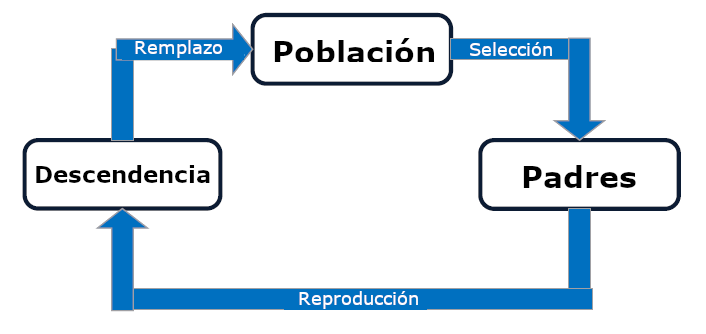
\includegraphics[width=8cm]{imagenes/esquema_evolutivo.png}
	\caption{Esquema de algoritmo evolutivo \cite{grosan2011intelligent}.}
	\label{fig:esquema_evolutivo}
\end{figure}

% Usually grouped under the term evolutionary computation or evolutionary algorithms
% [1][4], we find the domains of genetic algorithms [9], evolution strategies
% [26][27], evolutionary programming [28] and genetic programming [29].
% They all share a common conceptual base of simulating the evolution of individual
% structures via processes of selection, recombination and mutation reproduction and
% thereby producing better solutions. The processes depend on the perceived performance
% of the individual structures as defined by the problem. The procedure is
% then iterated as illustrated in Figure 14.1.

\section{Algoritmos Genéticos}
\label{sec:algoritmos_geneticos}
Los algoritmos genéticos son algoritmos de búsqueda, que al igual que los evolutivos, están basados en la selección natural, pero en este caso también se utilizan comportamientos de la genética en la naturaleza. Estos combinan la supervivencia del mas apto entre estructuras basadas en strings (cadenas de caracteres) con un intercambio de información estructurada pero aleatorizada para, de esta manera, formar un algoritmo de búsqueda con un estilo similar al de la búsqueda humana. En cada generación, un nuevo grupo de criaturas artificiales (strings) es creado creada y representada mediante bits procedentes de sus antecesores y nuevas partes. A pesar de ser aleatorios, los algoritmos genéticos no son simples búsquedas aleatorias. Estos aprovechan la información histórica para encontrar nuevos puntos de búsqueda de los que se espera una mejora con respecto a los anteriores \cite{goldberg1989genetic}.

Los algoritmos genéticos son probablemente el tipo de algoritmos evolutivos mas utilizados y simple de implementar para cualquier tipo de problema de optimización. Estos presentan diferentes maneras de diseñar la representación de los individuos, los mecanismos de selección y las operaciones de variación (recombinación y mutación) \cite{grosan2011intelligent}.

\subsection{Representación de Individuos}
La representación de los individuos es uno de los pasos mas importantes en el diseño de un algoritmo genético. La representación debe ser adecuada para el problema que se quiere resolver y debe consumir la menor cantidad de recursos posibles. Para un problema pueden haber múltiples posibles representaciones; por esto, tenemos que determinar cual es la mas adecuada para satisfacer las necesidades y requerimientos del problema \cite{grosan2011intelligent}.

Existen tipos estándar de representación de individuos, los cuales permiten utilizar la misma forma para diferentes problemas pero cambiando la interpretación que se les da. Algunas de las mas importantes son las siguientes:
\begin{itemize}
    \item Representación Binaria.
    \item Representación Entera.
    \item Representación Real o Flotante.
    \item Representación basada en Orden o Permutación.
\end{itemize}

\subsection{Inicialización de la Población}
El próximo paso en el desarrollo de un algoritmo genético es la inicialización de la población. Esto significa dar un semilla para generar aleatoriamente un número dado de individuos teniendo en cuenta la codificación/representación elegida. Mientras se realiza la generación, existen posibilidades que algunos individuos puedan tener múltiples copias de si mismos \cite{grosan2011intelligent}.

Para cada representación particular, existen diferentes técnicas para inicializar la población. Por ejemplo:

\begin{itemize}
    \item Para una representación binaria: un individuo esta representado por un string con valores de $\{0, 1\}$, por lo tanto los genes deberán inicializarse con valores $0$ o $1$ de manera equiprobable.
    \item Para una representación basada en orden: el individuo esta dado por una permutación de tamaño $n$. Cada gen $i$ deberá ser inicializado con valores entre $\{1, ..., n\}$ donde el valor no debe ocurrir en las posiciones previamente inicializadas.
\end{itemize}

\subsection{Mecanismos de Selección}
El proceso de selección en un algoritmo genético ocurre cuando los potenciales candidatos que para ser usados en el crossover son seleccionados. De manera estándar, los individuos mas aptos, con mayor \emph{fitness} a partir de ahora, son aquellos con mayor probabilidad de ser seleccionados \cite{grosan2011intelligent}.

Algunos de los mecanismo de selección mas utilizados son:

\begin{itemize}
    \item Selección por Torneo.
    \item Selección proporcional al fitness.
    \item Selección por Ruleta.
    \item Selección basada en Rango.
\end{itemize}

\subsection{Operaciones de Variación}
Las operaciones de variación principales son recombinación o \emph{crossover} y mutación. Cada una de ellas tienen formas especificas según las diferentes representaciones de individuos \cite{grosan2011intelligent}.

\subsubsection{Crossover o Recombinación}
El rol de la operación de \emph{crossover} es el de producir nuevos individuos combinando la información contenida en dos o mas padres. Esto se logra combinando los genes de los padres. Dependiendo en que representación estén dados tales genes, diferentes métodos serán utilizados y para estos también diferentes maneras de implementarlos \cite{grosan2011intelligent}: 

\begin{itemize}
    \item Recombinación binaria: crossover de un solo punto, crossover multi punto, crossover uniforme.
    \item Recombinación para enteros: pueden aplicarrse las mismas que en la recombinación binaria.
    \item Recombinación para reales: recombinación aritmética.
    \item Recombinación para representación basada en orden:  crossover mapeado parcialmente, crossover cíclico, crossover de borde.
\end{itemize}

\subsubsection{Mutación}
La mutación produce variaciones aleatorias sobre los individuos. Estas variaciones son por lo general pequeñas. La mutación se aplica a un individuo y puede producir solo un descendiente. Estas se aplican a los genes de un individuo, generalmente, con una baja probabilidad o ratio. Normalmente, los descendientes son mutados después de ser creados mediante crossover.

Como en el caso del crossover, la operación mutación toma varias formas dependiendo en la representación utilizada para los individuos y sobre cada una se pueden aplicar diferentes técnicas \cite{grosan2011intelligent}:

\begin{itemize}
    \item Mutación binaria: en esta representación solo se utilizan genes que pueden tomar dos valores, por lo que las mutaciones consisten en invertir algún gen elegido aleatoriamente con una cierta probabilidad.
    \item Mutación para enteros: reseteado aleatorio, mutación lenta.
    \item Mutación para reales: mutación uniforme, mutación no uniforme con distribución fija, 
    \item Mutación para representación basada en orden: mutación basada en intercambio, mutación basada en inserción, mutación \emph{Scramble} (mezclando), mutación basada en inversión.
\end{itemize}

\subsection{Modelos Poblacionales}
Existen dos modelos poblacionales definidos para algoritmos genéticos:

\subsubsection{Modelo Generacional}
En el modelo generacional, en cada generación el algoritmo empieza con una población de tamaño $N$. Un conjunto de apareamiento de tamaño $N$ es seleccionada a partir de este, donde algunos individuos serán seleccionados varias veces y otros no serán seleccionados en absoluto. Luego, se crean $N$ descendientes aplicando las operaciones de variación sobre estos. Después de cada generación la población es reemplazada por su descendencia, la cuál se transformará en la población de la siguiente generación \cite{grosan2011intelligent}.

\subsubsection{Modelo de Estado Estable}
En el modelo de estado estable, la población no es reemplazada en un paso. En este caso solo $M$ ($M<N$) individuos de la población anterior son reemplazados por nuevos individuos de la descendencia. El porcentaje de la población que es reemplazado es llamada ``brecha" generacional (o \emph{generational gap}) y es equivalente a $M/N$ \cite{grosan2011intelligent}. El algoritmo de estado estable es usualmente aplicado con $M=1$ y su correspondiente brecha generacional $1/N$ \cite{eiben2003introduction}.
% There are two main population models used by genetic algorithms:
% 1) Generational model and
% 2) Steady state model.
% Generational Model
% The generational model works as follows: in each generation the algorithm starts
% with a population of size N. A mating pool of size N is selected from this (some
% individuals will have multiple copies while other will not be selected at all). N
% offspring are further created by applying the variation operators. After each generation
% the whole population is replaced by the offspring population which will be
% the population of the next generation.
% Steady-state model
% In the steady-state model the population is not changed at once. In this case M
% (M<N) old individuals are replaced by M new individuals (from the offspring).
% The percentage of the population that is replaced is called generational gap and it
% is equal to M/N. The steady state algorithm has been widely applied especially
% with M=1 and the corresponding generational gap 1/N [2].

\subsection{Selección de Supervivientes y Reinserción}
Una vez que la descendencia ha sido producida mediante la selección, recombinación y mutación de los individuos de la población anterior, el fitness de la descendencia puede ser determinado. Si la descendencia producida tiene menor tamaño que la población original, entonces para mantener el tamaño de la población original, la descendencia debe ser reinsertada en la población anterior. Similarmente, si no toda la descendencia es utilizada en cada generación o si se generan mas individuos descendientes que el tamaño de la población anterior, entonces un esquema de reinserción debe ser utilizados para determinar que individuos existirán en la nueva población \cite{geatbx}.

Existen dos estrategias de reinserción principales:

% Once the offspring have been produced by selection, recombination and mutation
% of individuals from the old population, the fitness of the offspring may be determined.
% If less offspring are produced than the size of the original population then
% to maintain the size of the original population, the offspring have to be reinserted
% into the old population. Similarly, if not all offspring are to be used at each generation
% or if more offspring are generated than the size of the old population then a
% reinsertion scheme must be used to determine which individuals are to exist in the
% new population [12].
% There are two main reinsertion strategies:

\subsubsection{Reinserción Local}
En la reinserción local, los individuos son seleccionados en vecindarios o grupos delimitados. La reinserción de cada descendiente toma lugar en exactamente el mismo vecindario al que pertenece. En este sentido, la localidad de la información es preservada. El padre de algún individuo es el primero en ser seleccionado para ser padre del vecindario de este \cite{geatbx}.

Para la selección de padres existen a ser reemplazados y para la selección de descendencia para la reinserción existen varios esquemas posibles que toman algún criterio a partir del fitness de los individuos, o simplemente lo hacen de manera aleatoria. Un ejemplo sería: insertar la descendencia mas apta que los individuos menos aptos en el vecindario y reemplazar a los padres.
% In local selection, individuals are selected in a bounded neighborhood. The reinsertion
% of offspring takes place in exactly the same neighborhood. Thus, the locality
% of the information is preserved. The parent of an individual is the first selected
% parent in this neighborhood.
% For the selection of parents to be replaced and for selection of offspring to reinsert
% the following schemes are possible [12]:
\subsubsection{Reinserción Global}
Para la reinserción global existen diferentes esquemas \cite{geatbx}:

\begin{itemize}
    \item Reinserción pura: produce tanta descendencia como padres y reemplaza todos los padres por la descendencia.
    \item Reinserción uniforme: produce menos descendencia que padres y reemplaza los padres uniformemente al azar.
    \item Reinserción elitista: produce menos descendencia que padres y reemplaza los peores padres.
    \item Reinserción basada en el fitness: produce más descendencia que la necesaria y reinserta solamente los mejores individuos.
\end{itemize}

% • produce as many offspring as parents and replace all parents by the offspring
% (pure reinsertion);
% • produce less offspring than parents and replace parents uniformly at random
% (uniform reinsertion);
% • produce less offspring than parents and replace the worst parents (elitist
% reinsertion);
% • produce more offspring than needed for reinsertion and reinsert only the
% best offspring (fitness-based reinsertion).
% Pure reinsertion is the simplest reinsertion scheme. Every individual lives one
% generation only. This scheme is used in the simple genetic algorithm. However, it
% is very likely, that very good individuals are replaced without producing better
% offspring and thus, good information is lost.
% The elitist combined with fitness-based reinsertion prevents losing of information
% and is the recommended method. At each generation, a given number of the
% least fit parents are replaced by the same number of the most fit offspring. The fitness-
% based reinsertion scheme implements a truncation selection between offspring
% before inserting them into the population (i.e. before they can participate in the reproduction
% process). On the other hand, the best individuals can live for many generations.
% However, with every generation some new individuals are inserted. It is
% not checked whether the parents are replaced by better or worse offspring.
% Because parents may be replaced by offspring with a lower fitness, the average
% fitness of the population can decrease. However, if the inserted offspring are extremely
% bad, they will be replaced with new offspring in the next generation [12].

\subsection{Algoritmo Básico}
La forma básica de un algoritmo genético es la siguiente \cite{grosan2011intelligent}: \\

\noindent\emph{Paso 1} Generar una población aleatoria de $N$ cromosomas. \\
\emph{Paso 2} Evaluar cada cromosoma en la población utilizando la función de fitness. \\
\emph{Paso 3} Crear una nueva población repitiendo los siguientes pasos hasta que la nueva población este completa:
% The basic form of a general genetic algorithm is:
% Step 1 Generate random population of N chromosomes.
% Step 2 Evaluate each chromosome in the population using the fitness function
% Step 3 Create a new population by repeating following steps until the new
% population is complete
\begin{adjustwidth}{1.5cm}{}
\emph{Paso 3.1} Selección: selecciona dos cromosomas padres de la población de acuerdo con su fitness (cuanto mejor fitness, mayor es la posibilidad de ser seleccionado). \\
\emph{Paso 3.2} Crossover: dada un probabilidad de crossover, se cruzan a los padres para formar una nueva descendencia (hijos). Si no se realiza crossover, la descendencia es una copia exacta de los padres. \\
\emph{Paso 3.3} Mutación: dada una probabilidad de mutación, se mutan los individuos de la nueva descendencia en cada posición del cromosoma. \\
\emph{Paso 3.4} Reemplazo: se inserta la nueva descendencia en la población. \\
\end{adjustwidth}
% Step 3.1 Selection
% Select two parent chromosomes from a population according to their
% fitness (the better fitness, the higher the chance to be selected)
% Step 3.2 Crossover
% With a crossover probability cross over the parents to form new offspring
% (children). If no crossover was performed, offspring is the exact
% copy of parents.
% Step 3.3 Mutation
% With a mutation probability mutate new offspring at each locus (position
% in chromosome).
% Step 3.4 replacement
% Place new offspring in the new population
\emph{Paso 4} Utiliza la nueva población generada para nuevas generaciones (iteraciones) del algoritmo. \\
\emph{Paso 5} Si la condición de finalización es satisfecha, se detiene y retorna la mejor solución de la población actual. \\
\emph{Paso 6} Si no, retorna al \emph{Paso 2}. \\
% Step 4 Use new generated population for a further generation (iteration) of the
% algorithm
% Step 5 If the termination condition is satisfied, stop, and return the best solution
% in current population
% Step 6 Go to Step 2
\chapter{Diseño de los Algoritmos Propuestos}
\label{cap3}



En este capítulo se especifica el diseño de los dos algoritmos propuestos: el \emph{Algoritmo para Grafos Completos} y el \emph{Algoritmo ArcGen}. Ambos algoritmos tienen como  entrada grafos representados como \emph{Diagramas de Arcos} y su salida son grafos con menos cruces de arcos, esto es, permiten encontrar un grafo con óptimo \emph{crossing number}. Luego se muestra cómo estos algoritmos pueden integrarse con otros algoritmos de layout, o bien, servir como base para otras transformaciones sobre la representación del grafo.

\section{Algoritmo para Grafos Completos}
\label{sec:diseno_algoritmo_completo}
	%permite una representación del grafo de tal manera que los cruces que se obtenga de los nodos sean causa del orden de los nodos en una línea, y de la dirección (superior o inferior) que se le da al arco al dibujarlo, como puede observarse
	Debido  a la  simplicidad de los Diagramas de Arcos para esquematizar a los  grafos,  es que se  utiliza esta representación en busca de un grafo con una mínima cantidad de cruces de arcos.
	
	Así, se desarrolla  un algoritmo que permite visualizar  grafos  completos, es decir, aquellos donde cada par de vértices distintos está conectado por un arco, como un Diagrama de Arcos y que  soluciona el Crossing Number.
	%Inicialmente,  se plantea un método de ordenamiento que permita solucionar el Crossing Number para grafos completos, es decir, donde todos sus nodos están conectados con arcos a los restantes nodos. 
    Dado que el  grafo es completo, todos  los vértices tienen la misma cantidad de arcos,  luego se considera que todos los nodos poseen el mismo peso o importancia en el grafo. %Esto  no es posible ponderar a los nodos. no se diferencian de los demás.

	
	%figura mostrando K6 no óptimo
	
	A partir de un grafo completo se  genera  el  Diagrama de Arcos correspondiente, con  el mejor ordenamiento tanto de posición de los nodos sobre la línea, como de la ubicación de los arcos en el  plano,  tal que el número de cruces de arcos sea minimal.
	
	A fin de lograr esta representación óptima de cruces, no es necesario tener en cuenta el orden de los nodos, ya que, todos disponen de la misma cantidad de arcos salientes. Por lo tanto, el algoritmo se centra en distribuir los arcos de manera que su disposición sea equitativa, tanto en el semiplano  superior como en el inferior.
	
	La distribución de arcos se realiza comenzando por  dibujar  todos los arcos de los nodos de los extremos de la  recta, iniciando por la izquierda. Aquellos del nodo en el extremo  izquierdo  se dibujan en el semiplano  superior y aquellos del  nodo en el extremo  derecho en el inferior. Luego se continua dibujando los arcos correspondientes a los  nodos inmediatos al  procesado anteriormente en sentido al  centro de la línea, esquematizando primero el del lado izquierdo y luego el derecho. En la Figura \ref{fig:arcdiagram_k6_no_optimo}\ se muestra como  se visualiza  un grafo completo de 6 nodos.
	
	\begin{figure}[h]
		\centering
		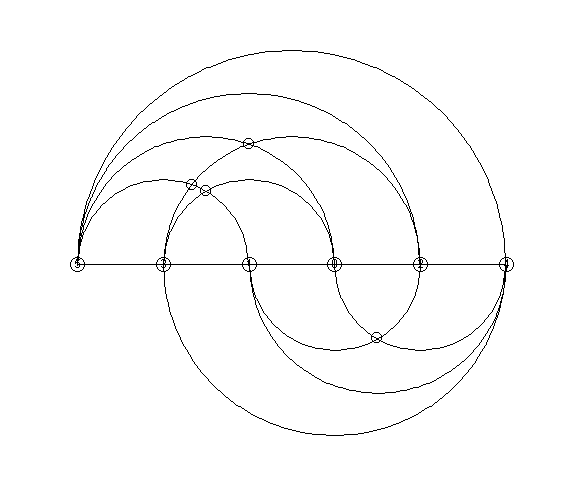
\includegraphics[width=8cm]{imagenes/grafo_1_bn.png}
		\caption{Diagrama de Arcos de un grafo completo de 6 nodos ($K_6$).}
		\label{fig:arcdiagram_k6_no_optimo}
	\end{figure}
	
	La  visualización  del grafo resultante de aplicar el algoritmo no resulta óptimo en cuanto a cantidad de cruces. Esto es posible de verificar debido a la conjetura que  plantea Guy en \cite{guy1960combinatorial},  que  da una cota superior para calcular el Crossing Number de grafos completos, notado $cr$,  y que proporciona un punto de referencia para medir la efectividad de nuestro algoritmo.
	
	$$cr(K_n) \leq \frac{1}{4} \floor*{\frac{n}{2}} \floor*{\frac{n-1}{2}} \floor*{\frac{n-2}{2}} \floor*{\frac{n-3}{2}}$$
	En nuestro  ejemplo, $cr(K_6)=3$ pero el dibujo del grafo  tiene 4 cruces.
	
	%A fin de resolver este problema, se buscaron los arcos que presentaban el problema, en grafos con diferentes cantidades de nodos. 
	
	A partir de la visualización de  una serie de grafos completos, se logra descubrir  que la aparición de cruces conflictivos  siguen un  patrón. En la Figura \ref{fig:arcdiagram_no_optimo} se presenta el patrón de los  arcos  conflictivos sobre cuatro grafos completos. 
	
	%podemos visualizar tal patrón, donde según el total de nodos podemos ver que se presentan más arcos conflictivos en lados opuestos, los cuales al invertirlos de sentido permiten eliminar los cruzamientos extras.
	
	\begin{figure}
		\centering
		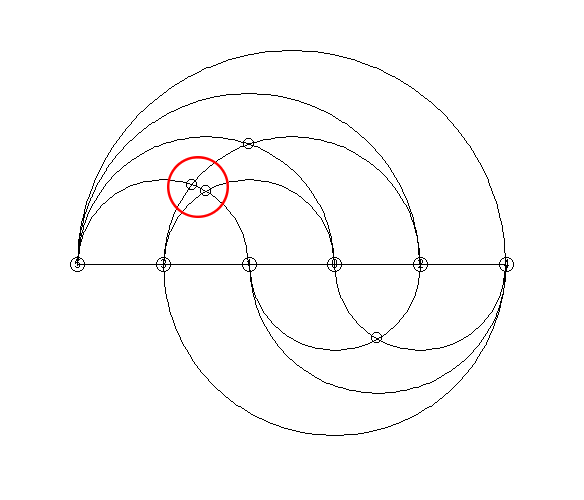
\includegraphics[width=8cm]{imagenes/grafo_1_bn_no_opt.png}
		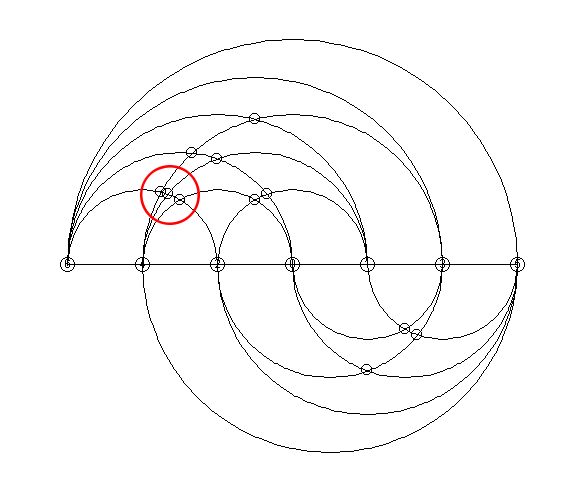
\includegraphics[width=7cm]{imagenes/grafo_2_bn_no_opt.png}\\
		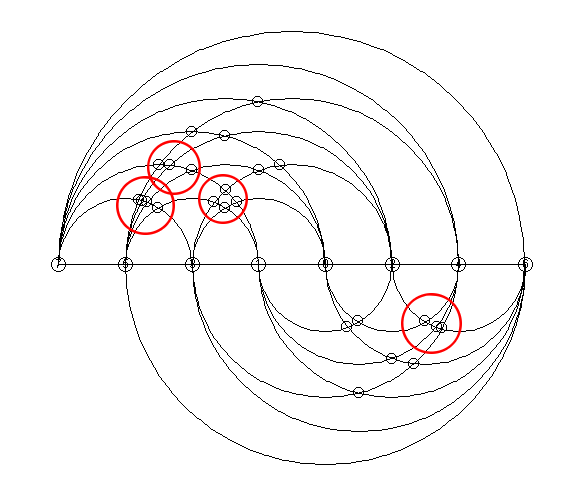
\includegraphics[width=7cm]{imagenes/grafo_3_bn_no_opt.png}
		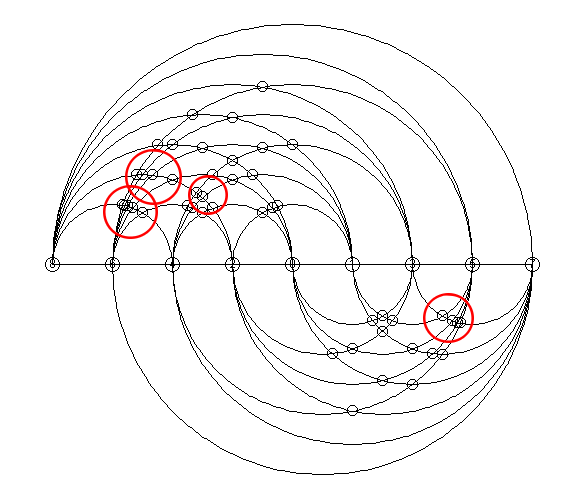
\includegraphics[width=7cm]{imagenes/grafo_4_bn_no_opt.png}
		\caption{Diagrama de Arcos de grafos completos $K_6$, $K_7$, $K_8$ y $K_9$ donde se puede visualizar cruces que siguen un patrón.}
		\label{fig:arcdiagram_no_optimo}
	\end{figure}
	
	%figura mostrando K6,K7,K8,K9 sin optimización
	
	Así, para solucionar el problema, se plantea una serie de transposiciones de arcos, cambiando el semiplano en donde está dibujado. El  número de transposiciones se determina según el patrón que siguen los grafos y  se calcula a partir de la cantidad de nodos, como:	$$t(n) = \floor*{\frac{n}{2}}-2,\ \mbox{con } n\geq 5.$$
	
	El algoritmo hace un recorrido sobre $t(n)$ nodos en la recta igual al de la distribución de los arcos en los semiplanos, comenzando en los extremos, esto es $$nodo_1, nodo_n, nodo_2, nodo_{n-1}, \ldots, nodo_{n / 2}$$ Para cada uno de los $t(n)$ nodos que recorre, se transponen $t(n), t(n)-1, t(n)-2, \ldots, 1$ arcos,  cambiando el  semiplano donde se dibujan, siempre que no aumente el número de cruces. Para el nodo actual $n_a$, los arcos a transponer se seleccionan ordenados por la cercanía que hay entre  $n_a$ y el nodo en el otro extremo del arco, esto es de izquierda a derecha sobre la línea recta desde $n_a$,  sin tener en cuenta el  arco que une a  $n_a$ con el siguiente en la recta. Consideremos al grafo completo $K_4$ de la Figura \ref{fig1:trasp} y sea $n_a=0$. Dado que el nodo 1 es el inmediato a 0, el arco (0,1) no es tenido en cuenta. El siguiente arco es el (0,2), por lo que éste es el que se transpone resultando el grafo  de la Figura \ref{fig2:trasp}.

    \begin{figure}
		\centering
		\subfigure[Grafo original completo $K_{4}$.]{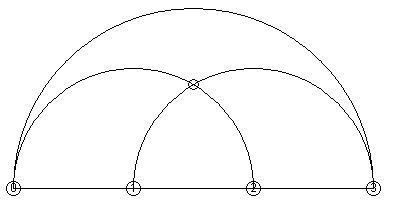
\includegraphics[width=9cm]{imagenes/ejemplo_transposicion_2.png}\label{fig1:trasp}}
		
		\subfigure[Grafo completo $K_{4}$ con el arco (0,2) transpuesto.]{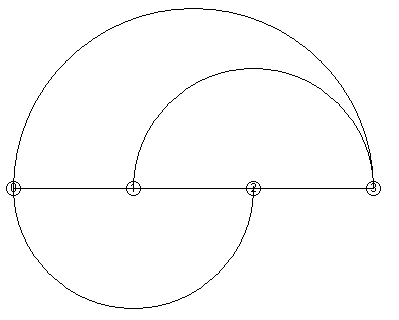
\includegraphics[width=9cm]{imagenes/ejemplo_transposicion_1.png}\label{fig2:trasp}}
		
		\caption{Dado un $n_a=0$ y el grafo completo $K_{4}$ el arco $(0,1)$ es ignorado para la transposición. En cambio se comienza la transposición con el arco $(0,2)$.}
		\label{fig:ejemplo_transposicion_completo}
	\end{figure}
	
	
	
	%a la generación de  transpone primero los $t(n)$ arcos conectados al nodo más próximo hacia el centro del grafo por el lado izquierdo, sin contar el nodo central (cuando $n$ es impar). Luego se saltea hacia el nodo en el extremo derecho y se reduce a  $t(n)-1$ siempre que sea positivo,  la cantidad de cambios, nuevamente invirtiendo desde el nodo mas próximo sin contar el primero. El proceso se repite con el nodo próximo al nodo del extremo izquierdo, y luego al próximo del extremo derecho y así sucesivamente, 
	En la Figura \ref{fig:arcdiagram_optimo}, se muestra el resultado de la  aplicación del proceso de  transposición.
	
	%	\todo[inline]{VER si lo ponemos: Este proceso se ha probado con grafos de más nodos, y se encontró en algunos casos que el cambio producía más cruces que los indicados por $cr(K_n)$ según la conjetura. Para solucionar esto se consideró evaluar los cruces de arcos antes y después de cambiar el arco de semiplano, y quedándose con el grafo que disponga menos. De esta manera el número $t(n)$ ya no determina la cantidad exacta de transposiciones de arcos sino que corresponde con una cota superior de transposiciones necesarias para la optimización.}
	
	\begin{figure}
		\centering
		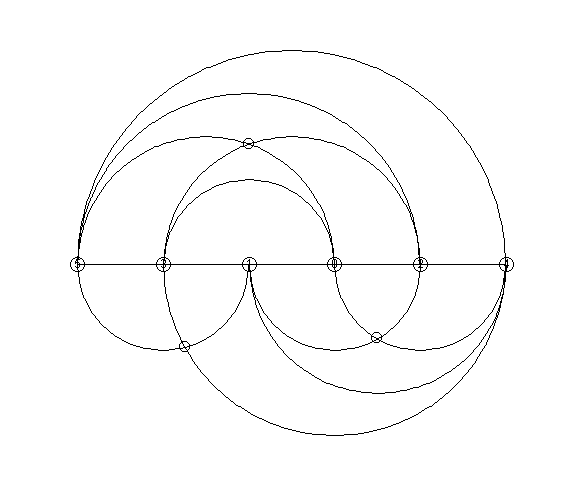
\includegraphics[width=7cm]{imagenes/grafo_1_bn_opt.png}
		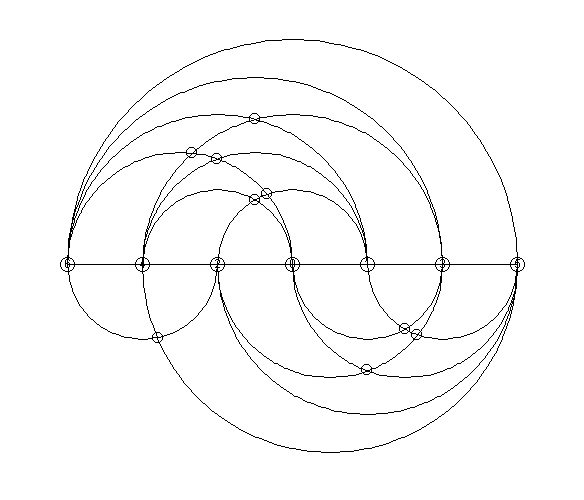
\includegraphics[width=7cm]{imagenes/grafo_2_bn_opt.png}\\
		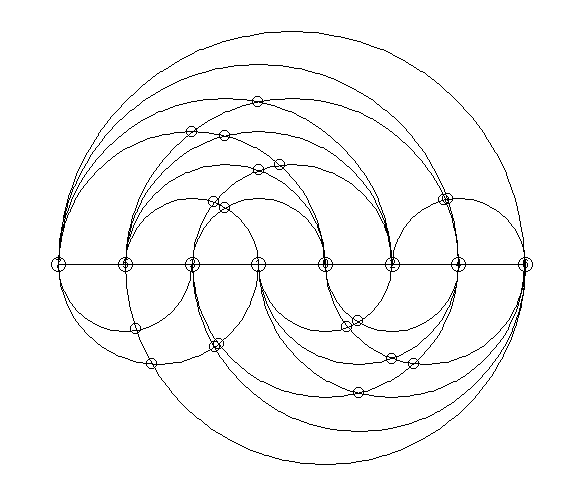
\includegraphics[width=7cm]{imagenes/grafo_3_bn_opt.png}
		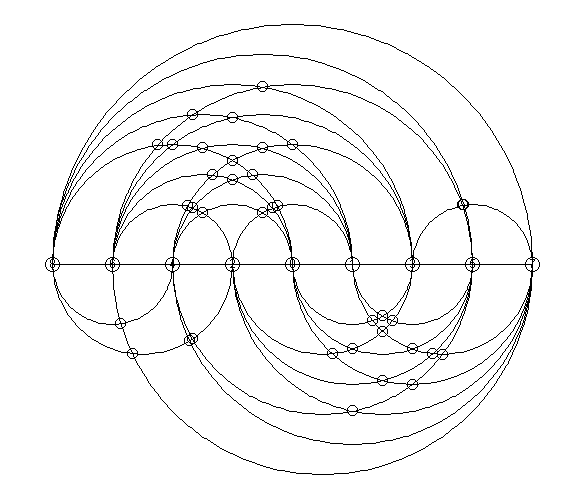
\includegraphics[width=7cm]{imagenes/grafo_4_bn_opt.png}
		\caption{Diagrama de Arcos de grafos completos $K_6$, $K_7$, $K_8$ y $K_9$ luego de solucionar los conflictos advertidos en la Figura \ref{fig:arcdiagram_no_optimo}.}
		\label{fig:arcdiagram_optimo}
	\end{figure}
	
	%figura mostrando K6,K7,K8,K9 con optimización
	
	Esta optimización nos permite obtener  una representación gráfica de un grafo completo con el mínimo Crossing Number, comparado con la conjetura dada. En forma empírica, esta  optimización  ha sido probada con el algoritmo hasta $K_{100}$.
	
	
	A partir de estos resultados,  se propone utilizar el algoritmo para un  grafo arbitrario, buscando que su Crossing Number sea minimal. Al permitir que los nodos puedan variar en cantidad de arcos, el algoritmo también debe tener en cuenta el orden de los mismos en la línea de nodos. A fin de  determinar un peso relativo para los nodos, dando un valor a partir del cuál se pueda proponer un orden para los nodos que obtenga un Crossing Number  mínimo o lo más bajo en lo posible, se introducen dos conceptos nuevos: Grado de Arco y Nivel de Nodo.
	
	%\begin{definition}[Grado de Nodo]
	%		El grado de un nodo se define como la cantidad de arcos que conectan con él.
	%	\end{definition}

	\begin{definition}[Grado de Arco]
		El grado de un arco se define como el grado de vértice (Definición \ref{defgradovertice}) más alto de los dos  que conecta. 
	\end{definition}
	
	El grado de arco permite dar una ponderación a cada arco según los nodos que conecta. De este  modo, se obtiene una cota superior en la cantidad de  nodos alcanzables desde los  extremos del arco.
	
	\begin{definition}[Nivel de Nodo]
		El nivel de un nodo se define como el grado de arco más bajo de los arcos que conectan con él.
	\end{definition}
	
	%Reordenamiento de  los nodos según el nivel del nodo.\\
	
	Intuitivamente,  el Nivel de Nodo permite determinar el  peso que tiene el nodo en el grafo, según sus relaciones con los demás nodos y así, da un criterio para ordenar los nodos del grafo en la recta,  antes de trazar los arcos. Un nodo con mayor conectividad se considera de mayor interés al  dibujar el grafo. %más interesante en un grafo, pero también es importante tener en cuenta el peso de las conexiones o arcos en sí mismas, para lo cuál se plantea el Grado de Arco, que surge del Grado de Nodo de los dos nodos que conecta. Este último se determina según la cantidad de arcos que salen de él, y permite al anterior dar una ponderación a cada arco según los nodos que conecta. Finalmente se define el nivel de nodo basado en los grados de sus arcos, para poder dar un peso al nodo con respecto a sus relaciones y al peso de las mismas.
	
	Dado el Nivel de Nodo se realiza un ordenamiento de los mismos de manera que aquellos con mayor nivel permanezcan lo más alejados posible entre ellos en la recta, buscando que se produzcan, de esta manera, la menor cantidad de cruzamientos entre sus arcos. Para ello se ubican en la recta los nodos en orden decreciente de nivel, ordenándolos en extremos opuestos del grafo de manera que queden lo más alejados del nodo anterior de mayor nivel y dejando aquellos de menor nivel en el centro del grafo, como se muestra en la Figura \ref{fig:arcdiagram_no_completo}.
	
	\begin{figure}
		\centering
		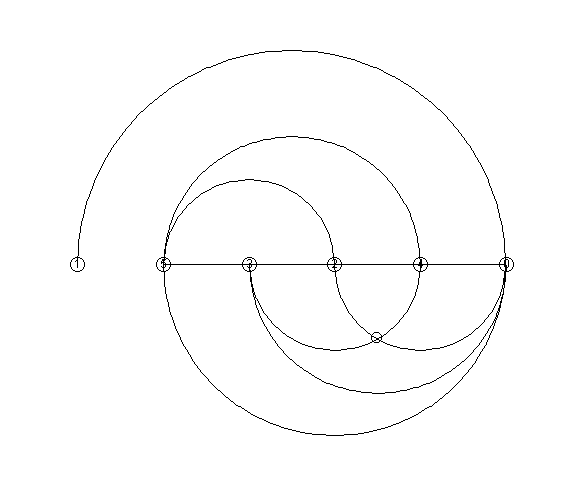
\includegraphics[width=7cm]{imagenes/grafo_aleatorio_6_nodos_bn.png}
		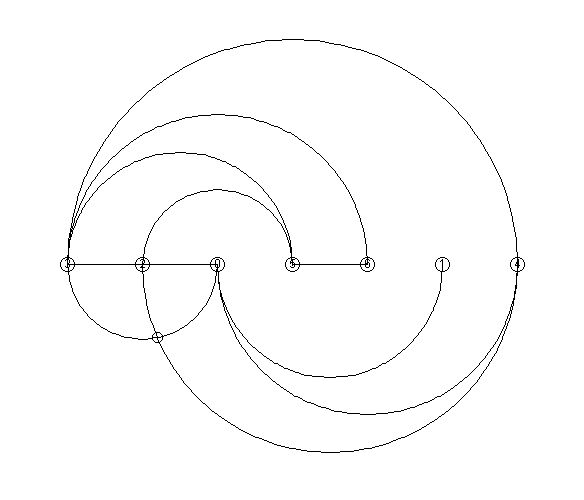
\includegraphics[width=7cm]{imagenes/grafo_aleatorio_7_nodos_bn.png}\\
		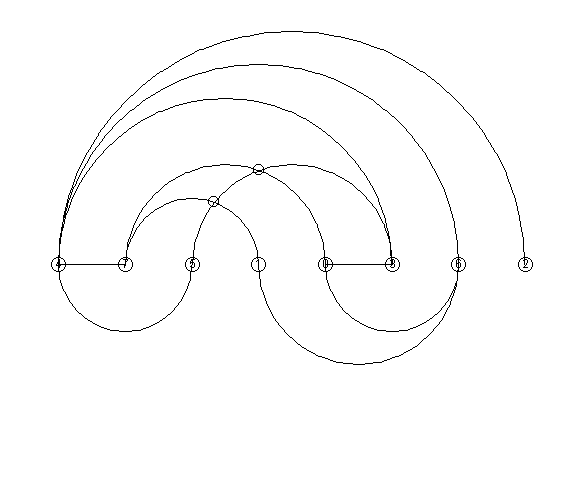
\includegraphics[width=7cm]{imagenes/grafo_aleatorio_8_nodos_bn.png}
		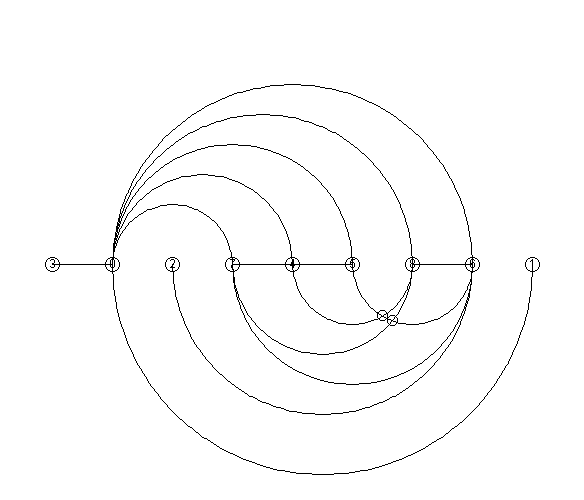
\includegraphics[width=7cm]{imagenes/grafo_aleatorio_9_nodos_bn.png}
		\caption{Diagrama de Arcos de grafos no completos generados aleatoriamente, en los cuáles se aplicó el algoritmo para Crossing Number mínimo en grafos completos.}
		\label{fig:arcdiagram_no_completo}
	\end{figure}
	
	%figura de ejemplo de Diagrama de Arcos no completo utilizando algoritmo optimo para completo
	
	Este criterio de ordenamiento junto con el algoritmo presentado anteriormente  para trazar los arcos, permiten obtener un Diagrama de Arcos con relativamente pocos cruces, pero que  no es óptimo  como lo era en grafos completos. Ya que los grafos no completos  no respetan el patrón de arcos en conflicto descubierto para los grafos completos, 
	no es posible aplicar la optimización descripta anteriormente.
	
	En conclusión, los algoritmos presentados  permiten  obtener un Diagrama de Arcos óptimo con respecto al Crossing Number en grafos completos, probado empíricamente hasta $K_{100}$, y relativamente bueno con respecto a grafos no completos. Esta visualización rectilínea de los grafos es el  punto de partida del algoritmo  que presentaremos en la siguiente sección para minimizar la cantidad de cruzamiento de arcos. 
	%para llegar a un resultado más satisfactorio con respecto a los cruzamientos de arcos y así acercarnos más a una mejor visualización, lo cuál es la finalidad de este trabajo.
	
	%Aplicación del algoritmo que devuelve un arc graph relativamente óptimo para  grafos completos con menor crossing
	%Un algoritmo  que permite que un grafo completo obtenga la menor cantidad de cruces,  hace que un grafo cualquiera tenga pocos cruces.

\section{Algoritmo ArcGen}
\label{sec:diseno_algoritmo_arcgen}

%	En la sección anterior hemos obtenido un Diagrama de Arcos, que a partir de un algoritmo sencillo y eficiente permite obtener un Crossing Number óptimo para arcos completos y uno relativamente bueno para grafos no completos. Ahora buscaremos optimizar estos últimos de manera que se pueda conseguir un resultado más satisfactorio, pero considerando algunas limitaciones en los grafos que trabajaremos.
	
	Motivados por una adecuada visualización de  modelos conceptuales, se diseñó   un nuevo algoritmo genético, considerando algunas limitaciones sobre los grafos que esquematizan estos diagramas, como el  hecho de que 
	%y diagramas de dominio que por lo general
	generalmente disponen de  grandes cantidades de entidades o clases (nodos del grafo), aunque disponen de cantidades moderadas o pequeñas de relaciones (arcos del grafo).
	El  algoritmo genético propuesto  mejora los resultados obtenidos con el algoritmo presentado en la sección anterior, que representa al grafo  con un Diagrama de Arcos. De hecho, este último se utiliza como un preprocesamiento sobre el grafo original,  para la generación de la población inicial del algoritmo genético.  Esto permite evolucionar  hacia  un grafo  con menos cruces (mínimo local) o  hacia el óptimo (mínimo número de cruces)  con  relativamente pocos cambios sobre el Diagrama de Arcos, y por lo tanto, obtener el resultado en  pocas generaciones. %Pero siempre buscando acotar el problema al objetivo que se planteó.
	
	\subsection{Representación de  los Individuos}
	\label{subsec:representacion_individuos}
	Cada individuo de la población corresponde a un Diagrama de Arcos. La representación incluye  los nodos y arcos del grafo, el orden de sus nodos sobre la línea (0 el nodo en el extremo izquierdo y  (n-1) el nodo en el extremo derecho) y el semiplano   (superior o inferior) en que se dibuja cada arco, como se muestra en la Figura \ref{fig:representacion_diagrama_arcos}.
	
	%\todo[inline]{Creo que no se requiere mantener dos arreglos  iguales.  Para que mantenes dos  arreglos iguales en distinto orden? No estoy segura que esto que corresponde más a implementación vaya acá}
	
	%\todo[inline,color=softred]{R: Esto debería ir en implementanción. Es por un tema de acceso, es por si necesitas acceder a un nodo por su posición o de su posición saber cuál es. (El nodo se identifica por un número)}
	
	%Para ello se mantiene  una estructura que dispone de un arreglo y una matriz de valores. 
	%%dos arreglos y una matriz de valores. El primer
	%El arreglo es un conjunto de nodos donde la posición del arreglo corresponde con el orden de los nodos sobre la recta de izquierda a derecha comenzando desde 0 hasta $n-1$ nodos, y el valor almacenado en cada posición corresponde con un número identificador del nodo. 
	%%El segundo arreglo es el inverso al primero, indicando en la posición el identificador del nodo y en el valor de la posición el orden del mismo. Finalmente 
	%La matriz es de $3\times m$ y cada columna representa uno de los $m$ arcos. La primer fila representa uno de los extremos del arco y la segunda el  otro extremo del arco. La tercer fila representa el semiplano donde se dibuja $0$ o $1$, que indica  el semiplano inferior o superior respectivamente, donde se grafica el arco. 
	
	
	%se corresponde con un conjunto de $m$ arcos donde en cada posición se almacenan tres valores, siendo dos de ellos los identificadores de los nodos que conecta y el tercer valor un número $0$ o $1$ correspondiente a la dirección (abajo o arriba) del arco gráficamente, y siendo la posición un identificador único del arco. 
	
	Teniendo en cuenta que  el grafo es  no dirigido, se considera que cada arco es único, es decir, solo se representa la relación de un nodo $n_i$ a un nodo $n_j$ y no la relación $n_j$ a $n_i$. Sin embargo, es posible extender la representación sin dificultad a digrafos.
	%buscar una estructura para que la representación sea eficiente (considerar como se muta)
	
	\begin{figure}
		\centering
		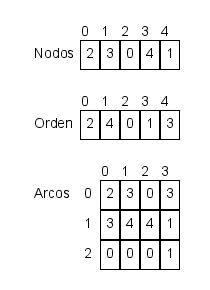
\includegraphics[width=4cm]{imagenes/representacion_ejemplo_1.png}
		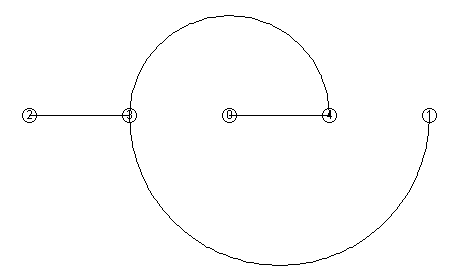
\includegraphics[scale=2.5]{imagenes/representacion_ejemplo_2.png}
		\caption{Estructura de datos para la representación de un Diagrama de Arcos.}
		\label{fig:representacion_diagrama_arcos}
	\end{figure}
	
	\subsection{Generación de Población Inicial}
	\label{subsec:generar_poblacion_inicial}
	La población inicial se genera a partir del Diagrama de Arcos obtenido del algoritmo explicado en la sección \ref{sec:diseno_algoritmo_completo}. 
	Para ello, se utiliza como semilla, al Diagrama de Arcos del  grafo  y  se realizan todas las posibles variaciones en un solo paso de orden de nodos y ubicación en los semiplanos de los arcos. Así, un posible individuo de la población inicial es la representación gráfica del grafo resultante de intercambiar el orden de dos nodos del Diagrama de Arcos, o de cambiar el semiplano donde se grafica  un arco particular, como se muestra en el ejemplo de la Figura \ref{fig:ejemplo_mutacion}.
	\begin{figure}
		\centering
		\subfigure[Grafo original generado aleatoriamente.]{
			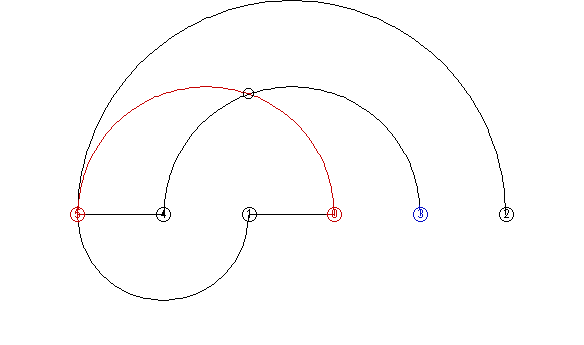
\includegraphics[scale=0.8]{imagenes/grafo_intercambio_original_bn.png}
			\label{subfig:ejemplo_mutacion_orig}
		}
		\subfigure[Grafo luego de intercambiar el nodo en la posición 0 por el de la posición 1.]{
			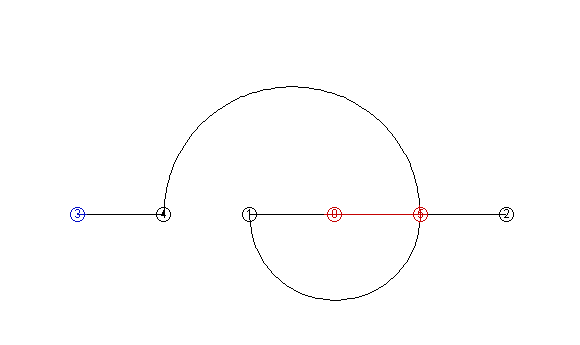
\includegraphics[scale=0.8]{imagenes/grafo_intercambio_nodo_bn.png}
			\label{subfig:ejemplo_mutacion_nodo}
		}
		\subfigure[Grafo luego de transponer el semiplano donde se grafica el arco entre los nodos en las posiciones 0 y 3.]{
			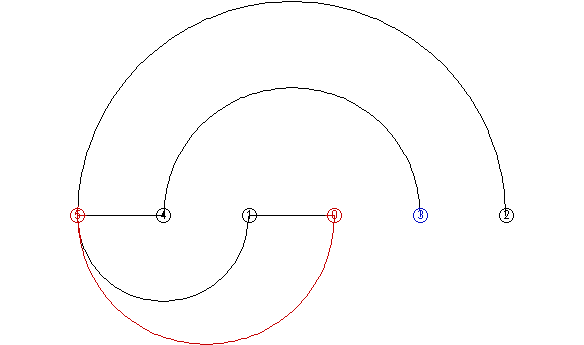
\includegraphics[scale=0.8]{imagenes/grafo_intercambio_arco_bn.png}
			\label{subfig:ejemplo_mutacion_arco}
		}
		\caption{Ejemplo de intercambio de nodos y cambio del semiplano donde se grafican los arcos.}
		\label{fig:ejemplo_mutacion}
	\end{figure}
	
	%figura de ejemplo mostrando un intercambio de nodos y un cambio de sentido de arco.
	
	Por lo tanto, la cantidad de individuos de la población inicial está dada por la siguiente fórmula:
	
	$$num_{P_0} = m+V^2_n= m+ \frac{n!}{(n-2)!}=m+n^2-n $$siendo $m$ la cantidad de arcos del grafo y $n$ la cantidad de nodos.
	
	\subsection{Mutación}
	\label{subsec:mutacion}
	El algoritmo  genético propuesto utiliza   mutación en sus individuos, pero  no se aplica crossover. Esta decisión de  diseño está basada en 
	algoritmos genéticos  con  objetivos similares \cite{he2007parallelisation, eloranta2001timga}. Sus autores especifican que  el crossover no es muy eficiente para resolver este problema, según los resultados experimentales obtenidos, por lo que se consideran porcentajes de mutación más altos y un crossover mínimo.
	%A partir del   relevamiento y análisis de algunos algoritmos genéticos  con  objetivos similares \cite{he2007parallelisation, eloranta2001timga}, en los cuáles se muestra que el crossover no es muy eficiente para este problema, según los resultados experimentales obtenidos, por lo que se proponen porcentajes de mutación más altos y un crossover mínimo.
	
	%En este sentido, para nuestro algoritmo se ha considerado anular el crossover y simplificar el problema a solo mutación. 
	Se proponen dos tipos de mutaciones posibles, con porcentajes basados en los utilizados en los trabajos \cite{he2007parallelisation, eloranta2001timga}:
	
	\begin{itemize}
		\item La primera mutación consiste en una transposición del  semiplano donde se grafica  un arco elegido al azar, como se muestra en la Figura \ref{subfig:ejemplo_mutacion_arco}. A está mutación se le ha dado un porcentaje de ocurrencia del 10\%.
		\item La segunda mutación consiste en el intercambio de orden de dos nodos elegidos al azar, como se muestra en la Figura \ref{subfig:ejemplo_mutacion_nodo}. A esta mutación se le ha dado un porcentaje de ocurrencia del 30\%.
	\end{itemize}
	
	Cada una de estas mutaciones,  son aplicadas a  cada individuo de la generación actual, buscando optimizar su Crossing Number.
	
	\subsection{Selección de Individuos}
	\label{subsec:seleccion_individuos}
	Una vez realizada la mutación del individuo se compara su Crossing Number (función de fitness) con el de la representación gráfica original del grafo y si aquel posee menos cruces se lo conserva y en caso contrario se lo descarta.
	%\todo[inline, color=orange]{GIULIANO VER}
	La  nueva población estará conformada por  individuos con un mejor layout que la  original del  grafo, aunque podría ser peor que el layout de su padre. Esto mantiene una población heterogénea.
	
	Por otra parte, nótese que por el criterio de selección de individuos la población varía su  tamaño,  de generación en generación. La población podría ser vacía si todos los hijos fueran peores que el layout original (semilla de la  población inicial),  dando así, un criterio extra para el  corte del  algoritmo.
	
	%A partir los individuos que se conserven se repite el proceso de mutación de la sección \ref{subsec:mutacion}.
	
	%\todo[inline,color=softred]{R: en respuesta a las dos anteriores. Si, la población es variable, en cada generación, cada individuo se compara con el original y si no lo mejora es eliminado de la población. Esto puede provocar que se extinga la población. Por lo que se guarda el mejor individuo que mejore al original y este es el que es retornado (o el original si ninguno lo mejoró).}
	
	\subsection{Criterio de Finalización del Algoritmo }
	%Se ha propuesto realizar varios ciclos (no son generaciones) del algoritmo genético para determinar su corte. Esto es,
	Dada la población inicial, primer generación, gestada  a partir de su Diagrama de Arcos, como se describe  en la sección \ref{subsec:generar_poblacion_inicial}, se realizan $1000$ generaciones en las cuáles tales individuos se mutan. Los individuos nuevos pueden ser eliminados de la  población, en caso de no superar el Crossing Number de la representación gráfica original del grafo.
	
	Una vez finalizadas las generaciones o extinta la población, se retorna el mejor Diagrama de Arcos obtenido y se comienza un nuevo ciclo utilizando este último como semilla generadora de la población inicial. Esto se repite hasta alcanzar un número máximo de ciclos  o cuando se iguala el número de cruces de  la mejor representación gráfica obtenida en dos ciclos consecutivos.
	
	%Un ciclo termina si se obtiene un Diagrama de Arcos sin cruces de arcos, o si se cumple con un número determinado de generaciones, o si la población se extingue, es decir ya no quedan individuos. En cualquiera de los casos se devolverá el mejor grafo obtenido o en caso de no mejorar el resultado, el mismo que se envío como entrada.
	
	%Mutación:
	%\begin{itemize}
	%    \item Intercambio de arco: arriba-abajo (10\%)
	%    \item Intercambio nodo al azar (30\%)
	%\end{itemize}
	
	%Argumentar  sobre los  porcentajes con el paper de paralelización
	
	%Cada  generación tiene una cantidad de $$m+V^2_n= m+ \frac{n!}{(n-2)!}=m+n^2-n $$ siendo  m cantidad de arcos y n cantidad de nodos
	
	%Los nodos con grado más alto probablemente sea  el centro del grafo. Si hubiera  más de un nodo  con alto grado  se deberán balancear.\\
	
	%Explicar la heurística: nro de cruces. 
	
	%Ejemplificar

\section{Integración con Algoritmos de Layout para Grafos Genéricos}
\label{sec:integracion_generico}
Los algoritmos presentados en secciones anteriores utilizan un estilo de dibujado de Diagrama de Arcos para representar a los individuos que computan. Esto es debido a la facilidad que este tipo de representación otorga para trabajar sobre el problema de crossing number para grafos. En contraparte el grafo resultante, a pesar de mejorar el crossing number original, no es apto para ser operado por un usuario final en una actividad de modelado, por lo que para poder finalizar el ciclo de estos algoritmos de layout y darle un uso práctico, es necesario realizar un último paso para transformar su estilo de dibujado en uno más intuitivo o genérico para que el usuario pueda visualizarlo fácilmente.

Existen varios algoritmos de layout que trabajan sobre grafos genéricos y que pueden servir para darle forma al grafo final que se busca obtener. En este sentido, el proceso se esquematiza como muestra la Figura \ref{fig:integracion_generico_diseno}, donde dado un grafo de entrada, se transforma el mismo en un diagrama de arcos para ser procesado por los algoritmos de este trabajo, luego al resultado se le realiza una transformación para adaptarlo al algoritmo que se utilizará finalmente para presentar el resultado como un grafo genérico.

\begin{figure}
	\centering
	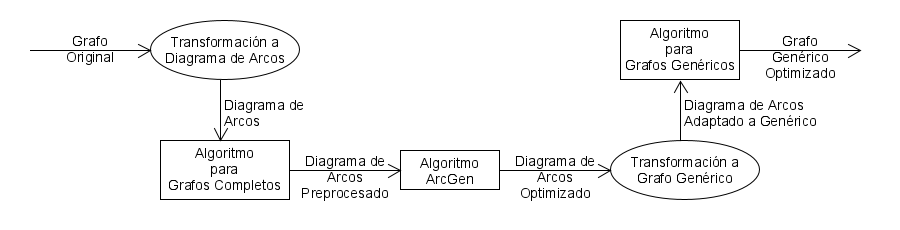
\includegraphics[width=16cm]{imagenes/integracion_generico_diseno.png}
	\caption{Esquema del proceso de aplicación de los algoritmos y su interacción con algoritmos para grafos genéricos.}
	\label{fig:integracion_generico_diseno}
\end{figure}

\subsection{Transformación de un Diagrama de Arcos en un Grafo Genérico}
\label{sec:transformacion_generico}
Para poder presentar el resultado final como un grafo genérico es necesario uno o varios procesos que realicen una transformación sobre el Diagrama de Arcos resultante y permita utilizarlo como entrada para algún otro algoritmo que dé la presentación final del grafo. Para este proceso hay que tener en cuenta que la representación que se utiliza para los individuos en el algoritmo para grafos completos y el algoritmo ArcGen, no explicita cómo se graficarán las aristas, más allá de su posición con respecto al semiplano y de que nodos conecta. En este sentido, al transformarse a un grafo genérico, es necesario agregar información extra a las aristas o a los nodos, ya sea indicando nuevos puntos para articular las líneas o indicando posiciones diferentes para los nodos. Cualquier cambio en la representación gráfica puede producir que el crossing number cambie.

Este proceso no necesariamente debe utilizar la información concebida como un Diagrama de Arcos, si no que puede visualizar los órdenes que se dieron a los nodos y la disposición de los arcos como información de base para ponderarlos y a partir de ello graficarlos mediante algún criterio ad hoc.
\chapter{Implementación de los Algoritmos Propuestos o  Implementación de ArcGen}\label{cap4}

\section{Herramientas y Lenguajes Utilizados}

\section{Aplicación de Algoritmos: Entorno de Prueba}
Los algoritmos presentados en las secciones \ref{sec:arcdiagram} y \ref{sec:genetico}, tanto el que obtiene un óptimo Crossing Number para grafos completos, como su refinamiento para grafos no completos y finalmente, \textsc{ArcGen}, el algoritmo genético para mejorar el resultado, fueron implementados en lenguaje Java. % y testeados. %A continuación veremos algunos pseudocódigos de estos algoritmos, los cuales utilizan un
	La  representación de Diagrama de Arcos % que se utiliza es la explicada dada en la sección \ref{subsec:representacion_individuos}. 
	%como se mencionó, registra tres arreglos donde
	almacena los nodos, su orden y sus arcos. Los métodos que incluye son: intercambiar nodos, mover un nodo a una posición realizando intercambios, transponer arcos, calcular cruces del grafo y de un arco en particular, calcular grado de arcos y nodos, y nivel de nodo y clonar el grafo.
	
    El algoritmo presentado en la Figura \ref{alg:arcdiagram_trazado}  realiza únicamente el trazado de los arcos como en la Figura \ref{fig:arcdiagram_k6_no_optimo}. Inicialmente,  ordena los nodos por su nivel. En  un grafo completo, el ordenamiento no produce ningún cambio, ya que todos sus nodos tienen el mismo nivel. Sin embargo, en los grafos no completos, permite un ordenamiento inicial más adecuado. Hay que considerar que el algoritmo realiza un recorrido desde el centro hacia los extremos a pesar de que la explicación inicial dada en la sección \ref{sec:arcdiagram} es a la inversa, esto es debido a la manera en que se da la implementación del Diagrama de Arcos y cómo se realizan los inversiones de arcos e intercambios de nodos internamente.
	Por último, el algoritmo invoca al algoritmo para optimizar grafos completos y eliminar los conflictos que genera.
	
	En el algoritmo descripto en la Figura \ref{alg:arcdiagram_optimizado} se presenta la optimización que soluciona los cruces conflictivos para grafos completos y permite obtener el Diagrama de Arcos inicial para lanzar el algoritmo genético.
	
	Finalmente,  se realiza la optimización con el algoritmo genético. El algoritmo presentado en la Figura \ref{alg:genetico} realiza las llamadas a cada ciclo de generaciones hasta encontrar dos ciclos con igual número de cruces o hasta cumplir con $100$ ciclos de tope. Cada ciclo es una llamada al algoritmo de 	generaciones [Figura \ref{alg:genetico_ciclo}], que genera poblaciones,  muta sus individuos, seleccionando los más aptos, \ \ esto es,\ \  aquellos 
		
	\begin{figure}
	    \begin{center}
		\begin{algorithmic}[1]
			\REQUIRE Diagrama de Arcos.
			\STATE Ordenar los nodos según su nivel en orden descendiente.
			\STATE Determina si el número de nodos ($n$) es par o impar.
			\STATE Asigna a un $punteroIzquierdo$ la posición $n/2$.
			\IF {número de nodos par}
			\STATE $punteroDerecho$ comenzará en $n/2 - 1 $.
			\ELSE
			\STATE $punteroDerecho$ comenzará en $n/2 + 1 $.
			\ENDIF
			\STATE Determina el semiplano inicial donde graficar. Si $n$ es par superior sino inferior.
			\FORALL {nodo $\in$ Nodos del grafo}
			\IF {semiplano es superior}
			\STATE Graficar todos los arcos del nodo en $punteroIzquierdo$ en semiplano superior.
			\ELSE 
			\STATE Graficar todos los arcos del nodo en $punteroDerecho$ en semiplano inferior.
			\ENDIF
			\STATE Invierte el semiplano para la próxima iteración.
			\ENDFOR
			\STATE Llamar a algoritmo para optimizar grafo completo con el grafo trazado como entrada.
			\ENSURE Diagrama de Arcos optimizado.
		\end{algorithmic}
	    \end{center}

		\caption{Pseudocódigo para el trazado inicial de un Diagrama de Arcos.}
		\label{alg:arcdiagram_trazado}
	\end{figure}
  
	\begin{figure}
	    \begin{center}
		\begin{algorithmic}[1]
			\REQUIRE Diagrama de Arcos trazado.
			\STATE Calcula el número de transposiciones $t(n) = \floor*{\frac{n}{2}}-2$, con $n > 5$, sino $0$ en caso de $n \leq 5$.
			\STATE Asigna a un $punteroIzquierdo$ la posición 0.
			\STATE Asigna a un $punteroDerecho$ la posición $n-1$.
			\STATE Comienza apuntando al $punteroIzquierdo$.
			\FOR {$i = 0$ hasta $t(n)$}
			\STATE Obtiene los arcos del nodo en el puntero que apunte.
			\STATE Cambia el puntero al opuesto.
			\STATE Inicializa $intercambios$ en $t(n)-i$.
			\WHILE {$j < $ arcos del nodo \AND $intercambios > 0$}
			\STATE Calcula el $CrossingNumber$ actual.
			\STATE Obtiene la $distancia$ entre el nodo actual y el nodo al que conecta el arco.
			\IF {$1 < distancia \leq (t(n)-i+1)$}
			\STATE Invierte el semiplano del arco[$j$].
			\STATE Recalcula el $CrossingNumber$.
			\IF {$CrossingNumber$ es mayor al anterior}
			\STATE Invierte el semiplano del arco[$j$] nuevamente.
			\ENDIF
			\ENDIF
			\ENDWHILE
			\ENDFOR
			\ENSURE Diagrama de Arcos optimizado.
		\end{algorithmic}
	    \end{center}

		\caption{Pseudocódigo para la optimización de Diagrama de Arcos completos.}
		\label{alg:arcdiagram_optimizado}
	\end{figure}
	
	\begin{figure}	
	    \begin{center}
		\begin{algorithmic}[1]
			\REQUIRE Diagrama de Arcos optimizado para completo, un entero $maxCiclos$.
			\STATE Asigna una variable $igualCrossNum$ en falso.
			\WHILE {$i < maxCiclos$ \AND $igualCrossNum$ sea falso}
			\STATE Llamar a algoritmo de ciclo genético y obtener un nuevo grafo.
			\IF {$CrossingNumber$ del grafo anterior es igual al nuevo}
			\STATE Asigna a $igualCrossNum$ verdadero.
			\ENDIF
			\ENDWHILE
			\ENSURE Diagrama de Arcos con optimización genética.
		\end{algorithmic}
	    \end{center}

		\caption{Pseudocódigo para la optimización genética de Diagrama de Arcos no completos.}
		\label{alg:genetico}
	\end{figure}
		\begin{figure}
	    \begin{center}
		\begin{algorithmic}[1]
			\REQUIRE Diagrama de Arcos de ciclo anterior, un entero $maxGeneraciones$.
			\STATE Calcula el $CrossingNumber$ del grafo de entrada, para comparar más adelante.
			\STATE Genera la población inicial con el grafo de entrada.
			\WHILE {$i < maxGeneraciones$ \AND grafo óptimo no encontrado}
			\FORALL {individuo de la población}
			\STATE Muta nodos del individuo con una probabilidad del 30\%.
			\STATE Muta arcos del individuo con una probabilidad del 10\%.
			\IF {individuo es un grafo óptimo (sin cruces)}
			\STATE Corta y devuelve el grafo óptimo.
			\ELSE
			\IF {individuo es peor que el original}
			\STATE Elimina al grafo de la población.
			\ENDIF
			\ENDIF
			\ENDFOR
			\IF {no se encontró grafo óptimo}
			\STATE Ordena los individuos por su fitness (menor CN).
			%\STATE Establece el mejor grafo obtenido de entre los individuos, considerando el mejor de las generaciones anteriores.
			\STATE Obtiene el primer individuo del conjunto (el de mejor fitness).
			% y verifica que tenga mejor fitness que el mejor obtenido en la generación anterior. Si es así lo establece como el mejor, caso contrario permanece el anterior.
			\IF {individuo tiene mejor fitness que mejor individuo de generaciones anteriores}
			\STATE Establece al nuevo individuo como el mejor obtenido.
			\ENDIF
			\ENDIF
			\ENDWHILE
			\ENSURE Diagrama de Arcos óptimo o mejor encontrado.
		\end{algorithmic}
	    \end{center}
		\caption{Pseudocódigo de un ciclo del algoritmo genético.}
		\label{alg:genetico_ciclo}
	\end{figure}
	
	%La generación de población inicial y procesos de mutación  son explicados en la sección \ref{sec:genetico}.
	\begin{figure}
		\centering
		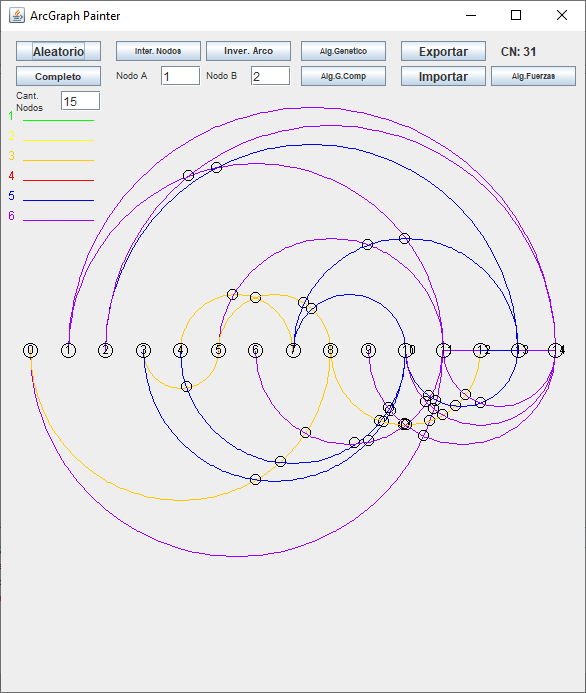
\includegraphics[width=8cm]{imagenes/aplicacion.png}
		\caption{Interfaz de la aplicación desarrollada para visualizar resultados y experimentación.}
		\label{fig:aplicacion}
	\end{figure}
	%Para probar los algoritmos explicados en las secciones anteriores se ha desarrollado una aplicación [Fig. \ref{fig:aplicacion}] que permite la visualización de los Diagrama de Arcos y por otro lado  almacena los resultados de tiempo, ciclos, arcos generados, cruces iniciales y finales de la ejecución del algoritmo genético, siendo que las optimizaciones anteriores son computables rápidamente.

	
	
	
	%\todo[inline,color=green]{COMPLETA}
	
\noindent con menor número de cruces que el grafo semilla y devuelve el mejor grafo obtenido.
	
		En la  Figura \ref{fig:aplicacion}, se muestra la interfaz  de la aplicación desarrollada  que permite la visualización de los Diagramas de Arcos.
		
			Los números en los nodos representan su nombre o identificador,  y permiten diferenciar al nodo sin considerar el 
	 orden en que se disponen en la recta del Diagrama de Arcos.
	
	Los arcos en el gráfico tienen diferentes colores de acuerdo a su Grado de Arco, según la definición dada en la sección \ref{sec:arcdiagram}, con el motivo de visualizar aquellos nodos con más relaciones, según los arcos que conecta.
	
	%\todo[inline,color=green]{COMPLETA idea de  los colores}
	
	%\todo[inline,color=green]{GIULIANO COMPLETA: La aplicación provee una serie de botones con los que se puede generar en forma aleatoria un grafo seteando  parámetros como  ..... los numeros de ExplicarInvertN,  InvertC}
	
	También se dispone de una serie de botones que brindan varias funcionalidades. Los botones \texttt{Random} y \texttt{Complete} permiten generar grafos aleatorio o completos, respectivamente, dada la cantidad de nodos que se especifican en una de las ventanas de texto. 
	
	Los botones \texttt{InvertN} y \texttt{InvertC} permiten invertir el orden de los nodos y transponer un arco dado entre dos nodos, respectivamente, obteniendo los identificadores de los nodos desde las ventanas de texto más pequeñas. 
	
	
	El botón \texttt{Genetic} permite lanzar el algoritmo genético \textsc{\textsc{ArcGen}} sobre el layout del grafo que se está visualizando actualmente, y lo reemplaza finalmente, por el layout resultante. Asimismo,  almacena los resultados de tiempo, ciclos, arcos generados, cruces iniciales y finales de la ejecución del algoritmo genético.
	
	Los botones \texttt{Export} e \texttt{Import} permiten exportar e importar un Diagrama de Arcos, utilizando un formato XML con una estructura propia de la aplicación.
	
	En la parte inferior encontramos los valores \texttt{Population}, \texttt{E.Time} y \texttt{E.Cycles} que indican el tamaño de la población, el tiempo y la cantidad de ciclos, estimados según los registros guardados para el algoritmo genético.	
	%\todo[inline]{almacena o  solo muestra???}
	
	%\todo[inline,color=softred]{R: los almacena, cada vez que se ejecuta el genetico guarda los datos de tiempo, ciclos, etc, y actualiza los valores que muestra en la aplicacion (que son promedios de los guardados).}
	%, siendo que las optimizaciones anteriores son computables rápidamente.
	
	La aplicación está  desarrollada bajo licencia libre y puede accederse a la versión más reciente de su ejecutable a través del repositorio de BitBucket  \url{https://bitbucket.org/giuliano-marinelli/graphlayout}.

\section{Integración con Algoritmo Dirigido por Fuerzas de Tunkelang}
\chapter{Resultados Experimentales}\label{cap5}
A fin de evaluar empíricamente los algoritmos implementados se han analizado sus comportamientos sobre grafos representados como diagramas de arcos, que fueron generados aleatoriamente. Se utilizó el ``número de nodos" como semilla para la generación aleatoria. Los arcos fueron generados aleatoriamente tanto en la posición de la curva sobre o por debajo del semiplano, como en los nodos que conectan, por lo que para una misma semilla (número de nodos) puede haber una cantidad variable de arcos que conectan diferentes nodos. 

En cada prueba se generaron 100 grafos para cada semilla, es decir 100 grafos aleatorios para cada número de nodos. Los resultados muestran los promedios de arcos generados, de tiempos y ciclos invertidos (para el caso del algoritmo genético) y de valores de crossing number inicial y final para cada semilla. 

En las pruebas mencionadas se utilizaron los mismos grafos aleatorios, es decir que sobre cada grafo original se aplicaron los algoritmos en diferentes ordenes y sucesiones de unos y otros, y de esta manera se pudo comparar el rendimiento de cada uno con respecto a los demás, como se muestra en la sección \ref{sec:resultados_finales}.

Estos resultados fueron obtenidos ejecutando un lote de pruebas sobre una computadora con procesador Intel Core i7-8650 de 2.11GHz, con una memoria RAM de 16GB y bajo un sistema operativo Windows 10 x64.

\section{Resultados de Algoritmo de Grafos Completos}
Esta prueba fue realizada a partir de aplicar el algoritmo para grafos completos, explicado en los capítulos anteriores, sobre un grafo original representado como diagrama de arcos que fue generado aleatoriamente como se explicó en la sección previa. En la figura \ref{fig:resultado_ejemplo_grafo_ori_lin} puede verse un ejemplo de aplicación del algoritmo. En la Tabla \ref{tab:resultados_orig_alg_com} pueden verse los promedios de tiempos de ejecución y de los crossing number resultantes comparados con los de los grafos originales para cada semilla.

\begin{figure*}[h]
	\centering
	\subfigure[Grafo original (CN: 209).]{
		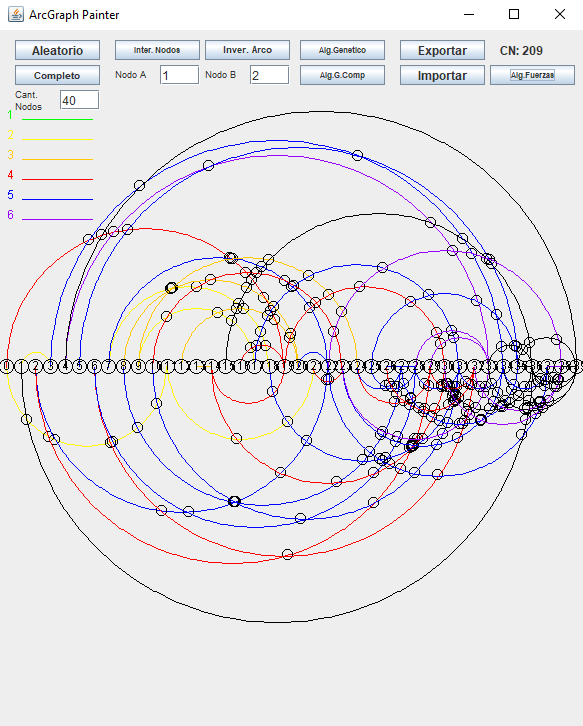
\includegraphics[width=0.45\textwidth]{imagenes/grafo_example_ori.png}
	}
	\subfigure[Grafo luego de aplicar algoritmo para grafos completos (CN: 123).]{
		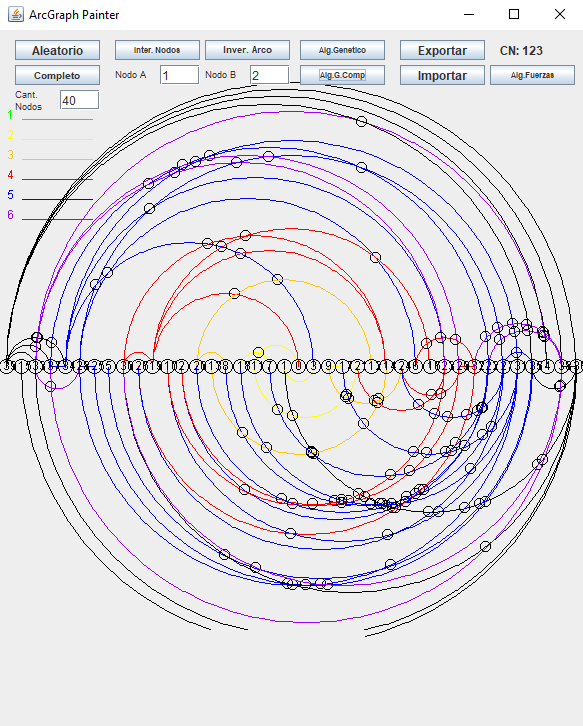
\includegraphics[width=0.45\textwidth]{imagenes/grafo_example_ori_lin.png}
	}
	\caption{Ejemplo de aplicar algoritmo para grafos completos sobre un grafo de 40 nodos aleatorio.}
	\label{fig:resultado_ejemplo_grafo_ori_lin}
\end{figure*}

\begin{table}[H]
	\caption{Promedios de 100 pruebas sobre cada semilla (de 5 a 50), del algoritmo para grafos completos sobre los grafos originales aleatorios.}
	\label{tab:resultados_orig_alg_com}
	\begin{tabularx}{\linewidth}{|p{1.5cm}|p{1.2cm}|p{1.5cm}|X|X|}
		\hline
		\multirow{2}{2cm}{\textbf{Nro. Nodos (semilla)}} & \multicolumn{4}{c|}{\textbf{Promedios}} \\
		\cline{2-5}
		& \textbf{Nro. Arcos} & \textbf{Tiempo} & \textbf{CN Grafo Origininal} & \textbf{CN Grafo Final} \\
		\hline
		10 & 13 & 0.000 s. & 7 & 3 \\
		\hline
		15 & 20 & 0.000 s. & 18 & 10 \\
		\hline
		20 & 28 & 0.001 s. & 38 & 23 \\
		\hline
		25 & 35 & 0.001 s. & 66 & 42 \\
		\hline
		30 & 43 & 0.001 s. & 103 & 63 \\
		\hline
		35 & 50 & 0.001 s. & 139 & 91 \\
		\hline
		40 & 58 & 0.001 s. & 195 & 123 \\
		\hline
		45 & 65 & 0.001 s. & 240 & 161 \\
		\hline
		50 & 73 & 0.002 s. & 312 & 198 \\
		\hline
	\end{tabularx}
\end{table}

\section{Resultados de Algoritmo ArcGen}
En estas pruebas se evalúan los resultados de aplicar el algoritmo genético ArcGen, explicado en los capítulos anteriores, sobre diferentes grafos de entrada.

\subsection{Resultados sobre Grafo Original}
Esta prueba aplica el algoritmo genético ArcGen sobre el grafo original generado aleatoriamente. En la figura \ref{fig:resultado_ejemplo_grafo_ori_gen} puede verse un ejemplo de aplicación del algoritmo. En la Tabla \ref{tab:resultados_orig_alg_gen} pueden verse los promedios de tiempos de ejecución, de las cantidades de ciclos y de los crossing number resultantes comparados con los de los grafos originales para cada semilla.

\begin{figure*}[h]
	\centering
	\subfigure[Grafo original (CN: 209).]{
		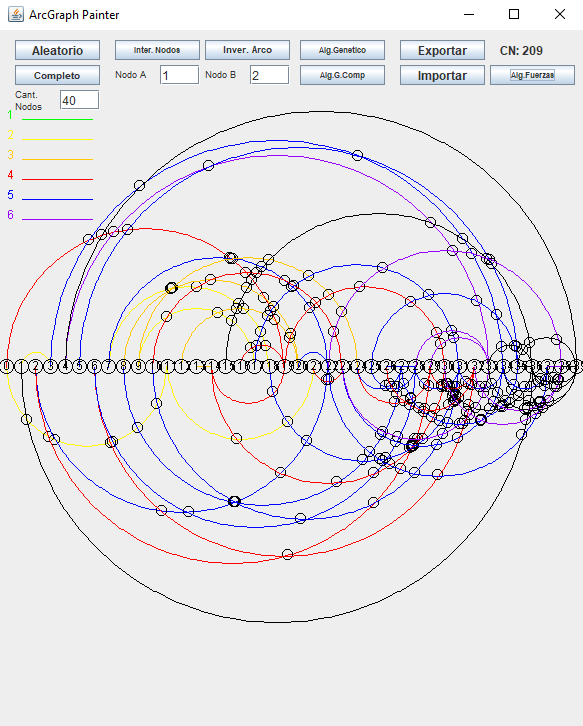
\includegraphics[width=0.45\textwidth]{imagenes/grafo_example_ori.png}
	}
	\subfigure[Grafo luego de aplicar algoritmo ArcGen (CN: 32).]{
		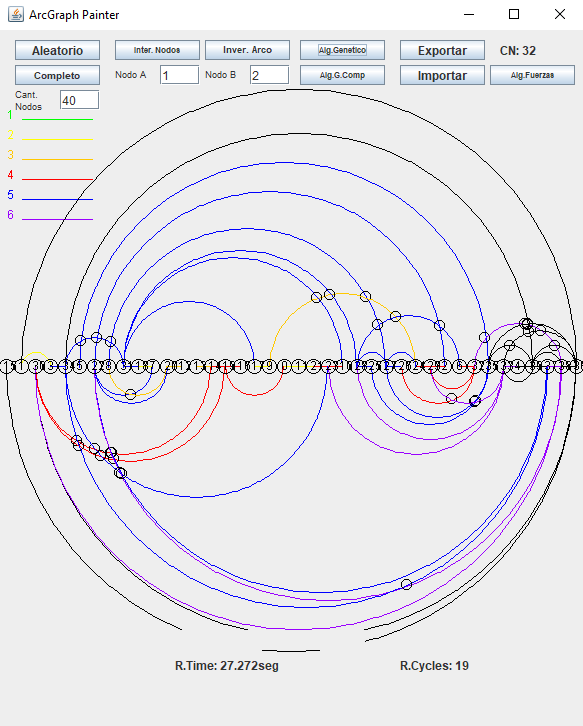
\includegraphics[width=0.45\textwidth]{imagenes/grafo_example_ori_gen.png}
	}
	\caption{Ejemplo de aplicar algoritmo ArcGen sobre un grafo de 40 nodos aleatorio.}
	\label{fig:resultado_ejemplo_grafo_ori_gen}
\end{figure*}

\begin{table}[H]
	\caption{Promedios de 100 pruebas sobre cada semilla (de 5 a 50), del algoritmo genético ArcGen sobre los grafos originales aleatorios.}
	\label{tab:resultados_orig_alg_gen}
	\begin{tabularx}{\linewidth}{|p{1.5cm}|p{1.2cm}|p{1.5cm}|p{1.5cm}|X|X|}
		\hline
		\multirow{2}{2cm}{\textbf{Nro. Nodos (semilla)}} & \multicolumn{5}{c|}{\textbf{Promedios}} \\
		\cline{2-6}
		& \textbf{Nro. Arcos} & \textbf{Tiempo} & \textbf{Ciclos} & \textbf{CN Grafo Original} & \textbf{CN Grafo Final} \\
		\hline
		10 & 13 & 0.024 s. & 2 & 7 & 0 \\
		\hline
		15 & 20 & 0.164 s. & 4 & 18 & 1 \\
		\hline
		20 & 28 & 0.613 s. & 7 & 38 & 4 \\
		\hline
		25 & 35 & 1.809 s. & 10 & 66 & 7 \\
		\hline
		30 & 43 & 10.953 s. & 13 & 103 & 12 \\
		\hline
		35 & 50 & 15.558 s. & 16 & 139 & 19 \\
		\hline
		40 & 58 & 15.921 s. & 20 & 195 & 27 \\
		\hline
		45 & 65 & 23.535 s. & 24 & 240 & 34 \\
		\hline
		50 & 73 & 45.778 s. & 28 & 312 & 43 \\
		\hline
	\end{tabularx}
\end{table}

\subsection{Resultados sobre Grafo Preprocesado por Algoritmo de Grafos Completos}
Esta prueba aplica el algoritmo genético ArcGen sobre el grafo original (generado aleatoriamente), luego de ser preprocesado por el algoritmo para grafos completos. En la figura \ref{fig:resultado_ejemplo_grafo_ori_lin_gen} puede verse un ejemplo de aplicación del algoritmo. En la Tabla \ref{tab:resultados_com_alg_gen} pueden verse los promedios de tiempos de ejecución, de las cantidades de ciclos y de los crossing number resultantes comparados con los de los grafos preprocesados para cada semilla.

\begin{figure*}[h]
	\centering
	\subfigure[Grafo preprocesado por algoritmo para grafos completos (CN: 123).]{
		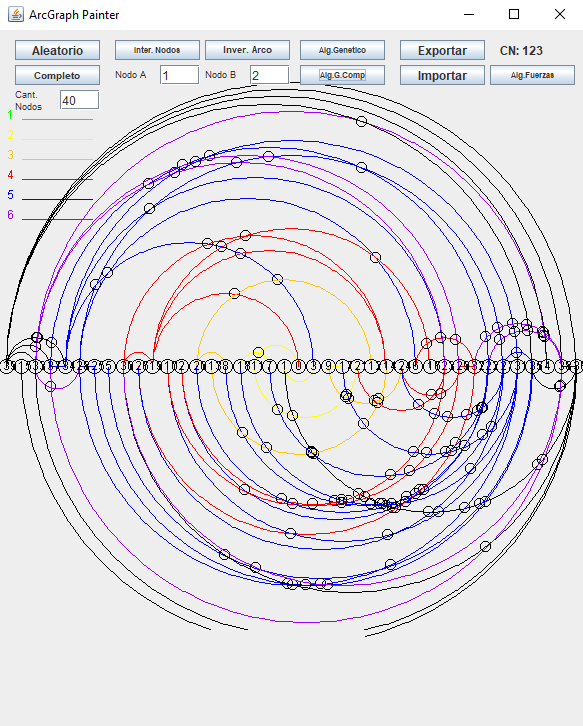
\includegraphics[width=0.45\textwidth]{imagenes/grafo_example_ori_lin.png}
	}
	\subfigure[Grafo luego de aplicar algoritmo ArcGen (CN: 39).]{
		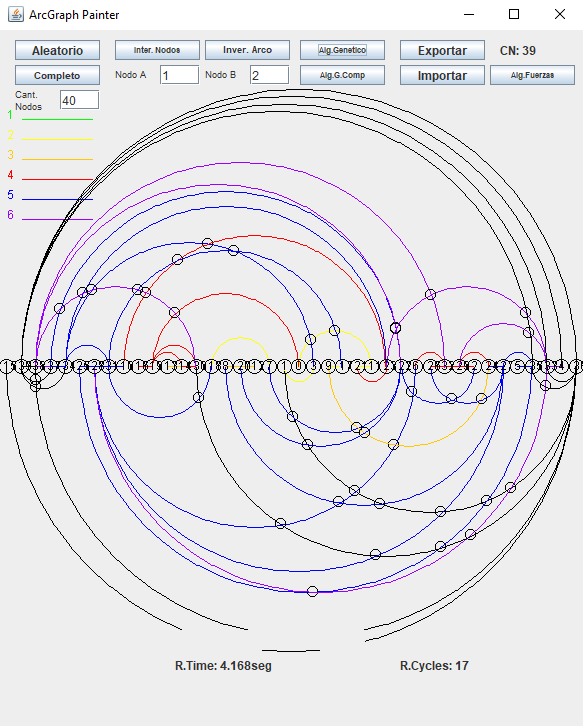
\includegraphics[width=0.45\textwidth]{imagenes/grafo_example_ori_lin_gen.png}
	}
	\caption{Ejemplo de aplicar algoritmo ArcGen sobre un grafo de 40 nodos aleatorio preprocesado por el algoritmo para grafos completos.}
	\label{fig:resultado_ejemplo_grafo_ori_lin_gen}
\end{figure*}

\begin{table}[H]
	\caption{Promedios de 100 pruebas sobre cada semilla (de 5 a 50), del algoritmo genético ArcGen sobre los grafos originales aleatorios preprocesados por el algoritmo para grafos completos.}
	\label{tab:resultados_com_alg_gen}
	\begin{tabularx}{\linewidth}{|p{1.5cm}|p{1.2cm}|p{1.5cm}|p{1.5cm}|X|X|}
		\hline
		\multirow{2}{2cm}{\textbf{Nro. Nodos (semilla)}} & \multicolumn{5}{c|}{\textbf{Promedios}} \\
		\cline{2-6}
		& \textbf{Nro. Arcos} & \textbf{Tiempo} & \textbf{Ciclos} & \textbf{CN Grafo Preprocesado} & \textbf{CN Grafo Final} \\
		\hline
		10 & 13 & 0.002 s. & 2 & 3 & 0 \\
		\hline
		15 & 20 & 0.023 s. & 4 & 10 & 1 \\
		\hline
		20 & 28 & 0.084 s. & 6 & 23 & 4 \\
		\hline
		25 & 35 & 0.308 s. & 9 & 42 & 8 \\
		\hline
		30 & 43 & 1.765 s. & 12 & 63 & 13 \\
		\hline
		35 & 50 & 2.757 s. & 14 & 91 & 20 \\
		\hline
		40 & 58 & 3.202 s. & 18 & 123 & 30 \\
		\hline
		45 & 65 & 6.152 s. & 21 & 161 & 39 \\
		\hline
		50 & 73 & 10.885 s. & 25 & 198 & 49 \\
		\hline
	\end{tabularx}
\end{table}

Dados los resultados de las tablas \ref{tab:resultados_orig_alg_gen} y \ref{tab:resultados_com_alg_gen} encontramos que el algoritmo ArcGen aplicado sobre el grafo preprocesado logra alcanzar un máximo local mucho más rápido que al aplicarse sobre el grafo original, pero a coste de que el máximo alcanzado sea menos óptimo.

\section{Resultados de Algoritmo de Fuerzas}
En estas pruebas se evalúan los resultados de aplicar el algoritmo dirigido por fuerzas de Tunkelang, sobre diferentes grafos de entrada.

\subsection{Resultados sobre Grafo Original}
Esta prueba aplica el algoritmo dirigido por fuerzas de Tunkelang sobre el grafo original generado aleatoriamente. En la figura \ref{fig:resultado_ejemplo_grafo_ori_fue} puede verse un ejemplo de aplicación del algoritmo. En la Tabla \ref{tab:resultados_orig_alg_fue} pueden verse los promedios de tiempos de ejecución y de los crossing number resultantes comparados con los de los grafos originales para cada semilla.

\begin{figure*}[h]
	\centering
	\subfigure[Grafo original (CN: 209).]{
		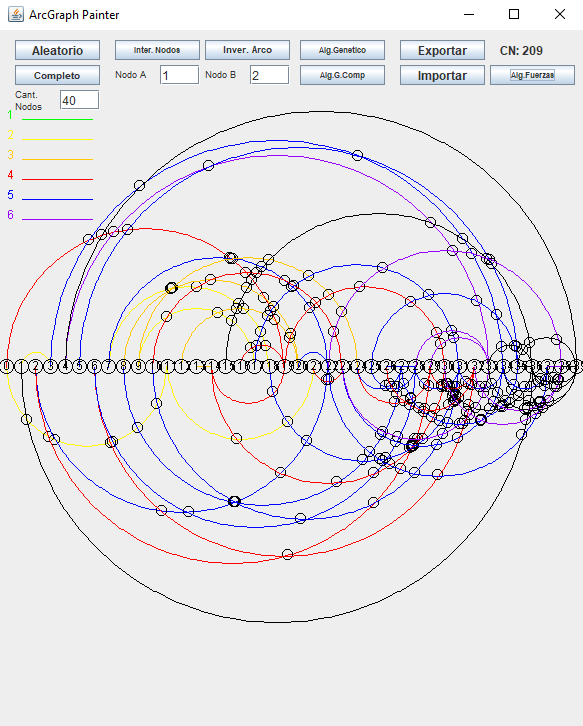
\includegraphics[width=0.45\textwidth]{imagenes/grafo_example_ori.png}
	}
	\subfigure[Grafo luego de aplicar algoritmo dirigido por fuerzas de Tunkelang (CN: 61).]{
		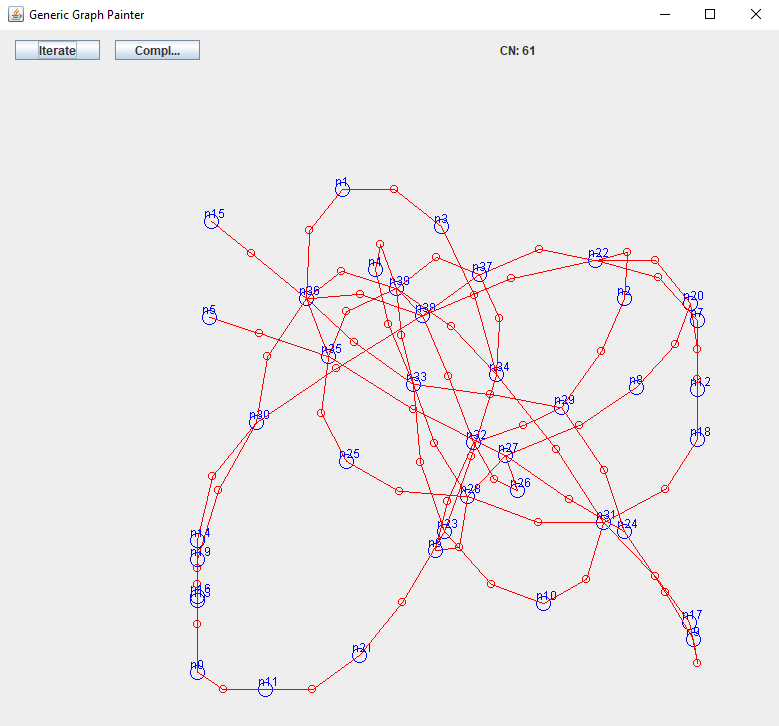
\includegraphics[width=0.5\textwidth]{imagenes/grafo_example_ori_fue.png}
	}
	\caption{Ejemplo de aplicar algoritmo dirigido por fuerzas de Tunkelang sobre un grafo de 40 nodos aleatorio.}
	\label{fig:resultado_ejemplo_grafo_ori_fue}
\end{figure*}

\begin{table}[H]
	\caption{Promedios de 100 pruebas sobre cada semilla (de 5 a 50), del algoritmo dirigido por fuerzas de Tunkelang sobre los grafos originales aleatorios.}
	\label{tab:resultados_orig_alg_fue}
	\begin{tabularx}{\linewidth}{|p{1.5cm}|p{1.2cm}|p{1.5cm}|X|X|}
		\hline
		\multirow{2}{2cm}{\textbf{Nro. Nodos (semilla)}} & \multicolumn{4}{c|}{\textbf{Promedios}} \\
		\cline{2-5}
		& \textbf{Nro. Arcos} & \textbf{Tiempo} & \textbf{CN Grafo Original} & \textbf{CN Grafo Final} \\
		\hline
		10 & 13 & 2.555 s. & 7 & 1 \\
		\hline
		15 & 20 & 2.525 s. & 18 & 3 \\
		\hline
		20 & 28 & 2.539 s. & 38 & 6 \\
		\hline
		25 & 35 & 2.546 s. & 66 & 10 \\
		\hline
		30 & 43 & 2.588 s. & 103 & 17 \\
		\hline
		35 & 50 & 2.593 s. & 139 & 24 \\
		\hline
		40 & 58 & 2.541 s. & 195 & 32 \\
		\hline
		45 & 65 & 2.527 s. & 240 & 42 \\
		\hline
		50 & 73 & 2.531 s. & 312 & 52 \\
		\hline
	\end{tabularx}
\end{table}

\subsection{Resultados sobre Grafo Preprocesado por Algoritmo de Grafos Completos}
Esta prueba aplica el algoritmo dirigido por fuerzas de Tunkelang sobre el grafo original (generado aleatoriamente), luego de ser preprocesado por el algoritmo para grafos completos. En la figura \ref{fig:resultado_ejemplo_grafo_ori_lin_fue} puede verse un ejemplo de aplicación del algoritmo. En la Tabla \ref{tab:resultados_com_alg_fue} pueden verse los promedios de tiempos de ejecución y de los crossing number resultantes comparados con los de los grafos preprocesados para cada semilla.

\begin{figure*}[h]
	\centering
	\subfigure[Grafo preprocesado por algoritmo para grafos completos (CN: 123).]{
		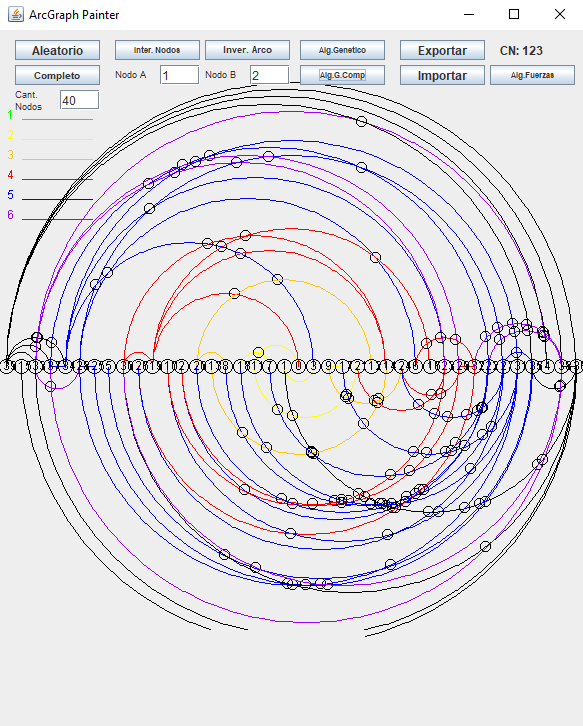
\includegraphics[width=0.45\textwidth]{imagenes/grafo_example_ori_lin.png}
	}
	\subfigure[Grafo luego de aplicar algoritmo dirigido por fuerzas de Tunkelang (CN: 49).]{
		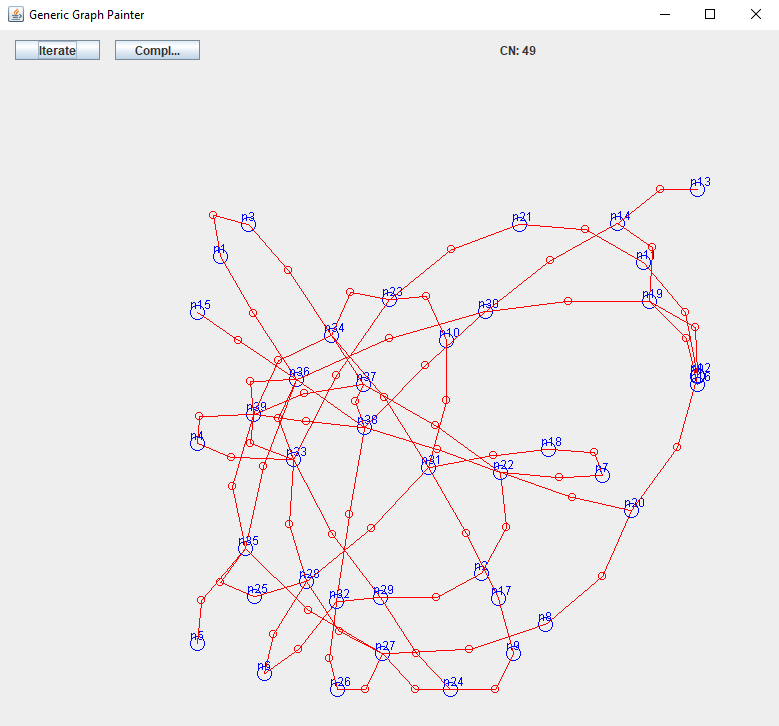
\includegraphics[width=0.5\textwidth]{imagenes/grafo_example_ori_lin_fue.png}
	}
	\caption{Ejemplo de aplicar algoritmo dirigido por fuerzas de Tunkelang sobre un grafo de 40 nodos aleatorio preprocesado por el algoritmo para grafos completos.}
	\label{fig:resultado_ejemplo_grafo_ori_lin_fue}
\end{figure*}

\begin{table}[H]
	\caption{Promedios de 100 pruebas sobre cada semilla (de 5 a 50), del algoritmo dirigido por fuerzas de Tunkelang sobre los grafos originales aleatorios preprocesados por el algoritmo para grafos completos.}
	\label{tab:resultados_com_alg_fue}
	\begin{tabularx}{\linewidth}{|p{1.5cm}|p{1.2cm}|p{1.5cm}|X|X|}
		\hline
		\multirow{2}{2cm}{\textbf{Nro. Nodos (semilla)}} & \multicolumn{4}{c|}{\textbf{Promedios}} \\
		\cline{2-5}
		& \textbf{Nro. Arcos} & \textbf{Tiempo} & \textbf{CN Grafo Preprocesado} & \textbf{CN Grafo Final} \\
		\hline
		10 & 13 & 2.557 s. & 3 & 0 \\
		\hline
		15 & 20 & 2.527 s. & 10 & 2 \\
		\hline
		20 & 28 & 2.537 s. & 23 & 6 \\
		\hline
		25 & 35 & 2.545 s. & 42 & 10 \\
		\hline
		30 & 43 & 2.589 s. & 63 & 17 \\
		\hline
		35 & 50 & 2.593 s. & 91 & 23 \\
		\hline
		40 & 58 & 2.543 s. & 123 & 31 \\
		\hline
		45 & 65 & 2.527 s. & 161 & 41 \\
		\hline
		50 & 73 & 2.536 s. & 198 & 51 \\
		\hline
	\end{tabularx}
\end{table}

\subsection{Resultados sobre Grafo Preprocesado por Algoritmo ArcGen}
Esta prueba aplica el algoritmo dirigido por fuerzas de Tunkelang sobre el grafo original (generado aleatoriamente), luego de ser preprocesado por el algoritmo ArcGen. En la figura \ref{fig:resultado_ejemplo_grafo_ori_gen_fue} puede verse un ejemplo de aplicación del algoritmo. En la Tabla \ref{tab:resultados_gen_alg_fue} pueden verse los promedios de tiempos de ejecución y de los crossing number resultantes comparados con los de los grafos preprocesados para cada semilla.

\begin{figure*}[h]
	\centering
	\subfigure[Grafo preprocesado por algoritmo ArcGen (CN: 32).]{
		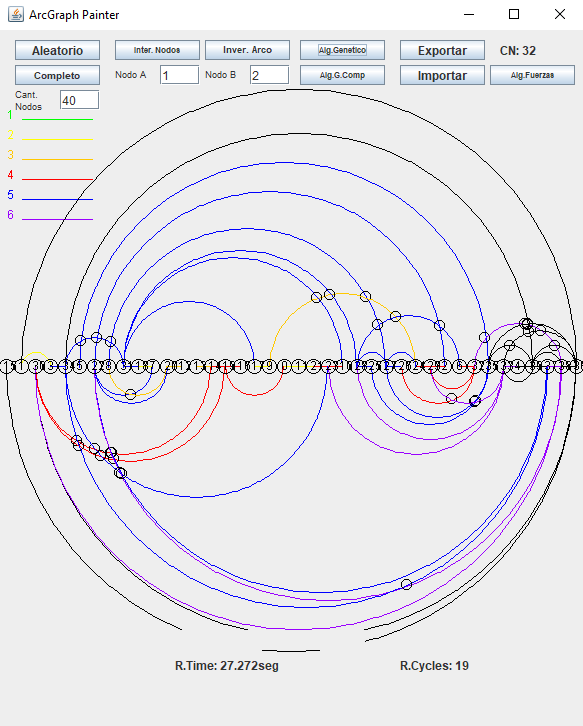
\includegraphics[width=0.45\textwidth]{imagenes/grafo_example_ori_gen.png}
	}
	\subfigure[Grafo luego de aplicar algoritmo dirigido por fuerzas de Tunkelang (CN: 34).]{
		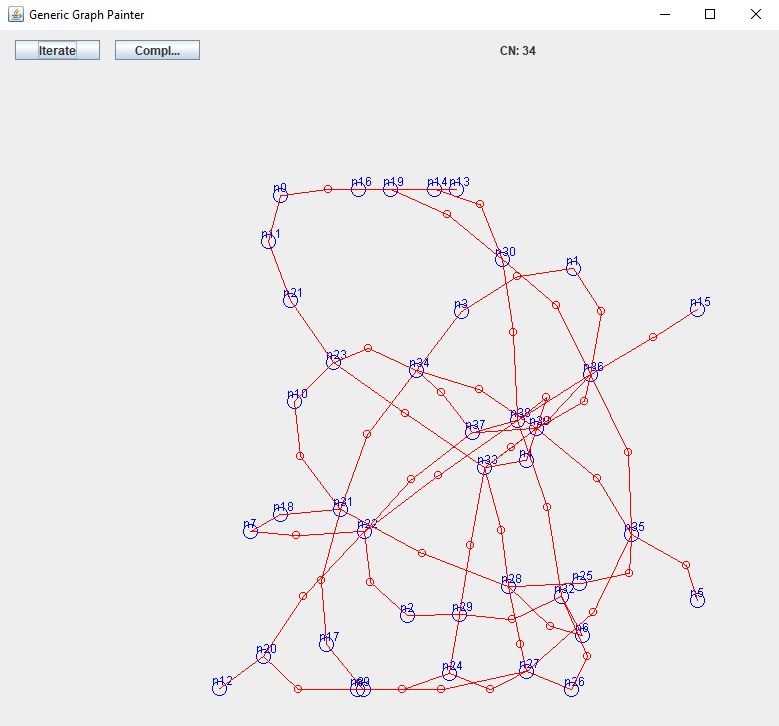
\includegraphics[width=0.5\textwidth]{imagenes/grafo_example_ori_gen_fue.png}
	}
	\caption{Ejemplo de aplicar algoritmo dirigido por fuerzas de Tunkelang sobre un grafo de 40 nodos aleatorio preprocesado por el algoritmo ArcGen.}
	\label{fig:resultado_ejemplo_grafo_ori_gen_fue}
\end{figure*}

\begin{table}[H]
	\caption{Promedios de 100 pruebas sobre cada semilla (de 5 a 50), del algoritmo dirigido por fuerzas de Tunkelang sobre los grafos originales aleatorios preprocesados por el algoritmo ArcGen.}
	\label{tab:resultados_gen_alg_fue}
	\begin{tabularx}{\linewidth}{|p{1.5cm}|p{1.2cm}|p{1.5cm}|X|X|}
		\hline
		\multirow{2}{2cm}{\textbf{Nro. Nodos (semilla)}} & \multicolumn{4}{c|}{\textbf{Promedios}} \\
		\cline{2-5}
		& \textbf{Nro. Arcos} & \textbf{Tiempo} & \textbf{CN Grafo Preprocesado} & \textbf{CN Grafo Final} \\
		\hline
		10 & 13 & 2.577 s. & 0 & 0 \\
		\hline
		15 & 20 & 2.691 s. & 1 & 2 \\
		\hline
		20 & 28 & 3.166 s. & 4 & 5 \\
		\hline
		25 & 35 & 4.352 s. & 7 & 9 \\
		\hline
		30 & 43 & 13.511 s. & 12 & 15 \\
		\hline
		35 & 50 & 18.140 s. & 19 & 22 \\
		\hline
		40 & 58 & 18.464 s. & 27 & 27 \\
		\hline
		45 & 65 & 26.062 s. & 34 & 37 \\
		\hline
		50 & 73 & 48.312 s. & 43 & 46 \\
		\hline
	\end{tabularx}
\end{table}

\section{Resultados Finales}
\label{sec:resultados_finales}
Finalmente se realiza la prueba completa, utilizando sobre el grafo original, el algoritmo para grafos completos, seguido por el algoritmo ArcGen y finalmente el algoritmo dirigido por fuerzas de Tunkelang. En la figura \ref{fig:resultado_ejemplo_grafo_ori_lin_gen_fue} puede verse un ejemplo del resultado final de aplicar todos los algoritmos. En la Tabla \ref{tab:resultados_orig_alg_com_gen_fue} pueden verse los promedios de tiempos de ejecución y de los crossing number resultantes para cada semilla. Luego, en la Tabla \ref{tab:resultados_comparacion} se comparan los resultados obtenidos anteriormente por el algoritmo de fuerzas con los resultados de esta prueba.

\begin{figure*}[h]
	\centering
	\subfigure[Grafo original (CN: 209).]{
		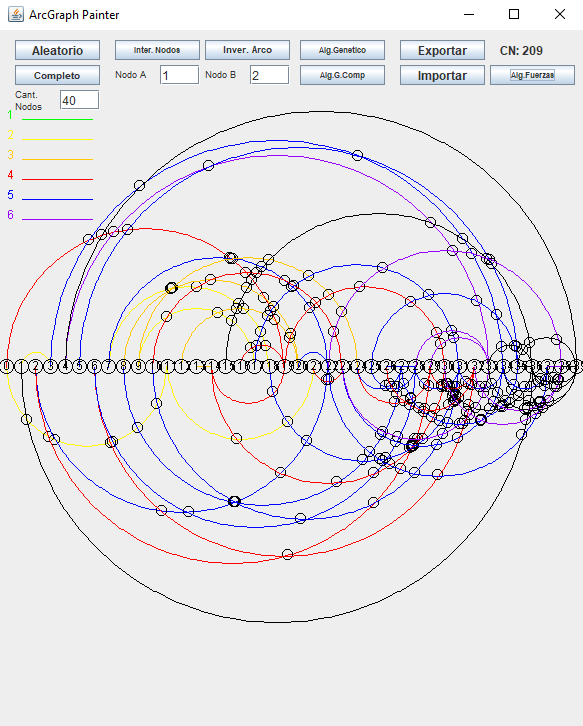
\includegraphics[width=0.45\textwidth]{imagenes/grafo_example_ori.png}
	}
	\subfigure[Grafo luego de aplicar el algoritmo para grafos completos, seguido del algoritmo ArcGen y finalmente el algoritmo dirigido por fuerzas de Tunkelang (CN: 34).]{
		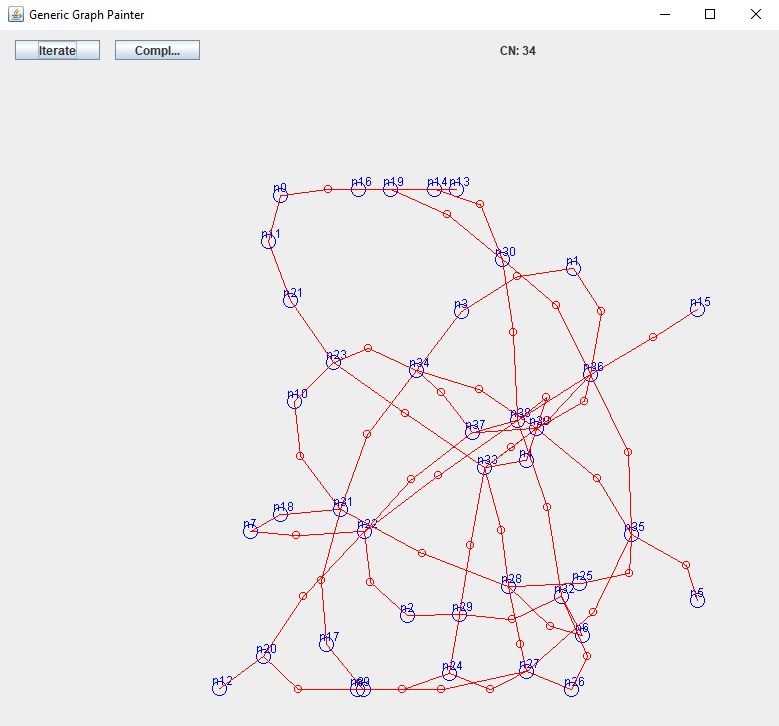
\includegraphics[width=0.5\textwidth]{imagenes/grafo_example_ori_gen_fue.png}
	}
	\caption{Ejemplo de aplicar algoritmo dirigido por fuerzas de Tunkelang sobre un grafo de 40 nodos aleatorio preprocesado por el algoritmo ArcGen y por algoritmo para grafos completos.}
	\label{fig:resultado_ejemplo_grafo_ori_lin_gen_fue}
\end{figure*}

%La Tabla \ref{tab:resultados_exp}\ presenta los promedios mencionados de los resultados recopilados de las ejecuciones del algoritmo genético sobre grafos generados en forma aleatoria, con diferentes cantidades de nodos. 

%	 La recopilación de resultados de ejecuciones del algoritmo genético sobre grafos generados aleatoriamente con diferentes cantidades de nodos y de estos se han obtenido promedios. Esta muestra los promedios de $100$ ejecuciones para cada número de nodos.


%Procesador sobre el que se corre.\\
%En general  trabajamos con modelos conceptuales que no tienen normalmente más de 4 arcos(relaciones entre los  nodos) por nodo (nodos conceptos o  clases o entidades)  

%Tenemos probablemente muchas clases (nodos)\\

%Teniendo en cuenta que la motivación del desarrollo de este algoritmo de layout es su incorporación y utilización en herramientas gráficas de modelado conceptual  y que generalmente los modelos no contienen  grandes cantidades de nodos, los test realizados sobre la aplicación  se han limitado a un máximo de 50 nodos.
\begin{table}[H]
	\caption{Promedios de 100 pruebas sobre cada semilla (de 5 a 50), del algoritmo dirigido por fuerzas de Tunkelang sobre los grafos originales aleatorios preprocesados, primero por el algoritmo para grafos completos y luego por el algoritmo ArcGen.}
	\label{tab:resultados_orig_alg_com_gen_fue}
	\begin{tabularx}{\linewidth}{|p{1.5cm}|p{1.2cm}|p{1.5cm}|p{1.5cm}|X|X|}
		\hline
		\multirow{2}{2cm}{\textbf{Nro. Nodos (semilla)}} & \multicolumn{5}{c|}{\textbf{Promedios}} \\
		\cline{2-6} & \textbf{Nro. Arcos} & \textbf{Tiempo} & \textbf{Ciclos} & \textbf{CN Inicial} & \textbf{CN Final} \\
		\hline
		10 & 13 & 2.556 s. & 2 & 7 & 0 \\
		\hline
		15 & 20 & 2.551 s. & 4 & 18 & 2 \\
		\hline
		20 & 28 & 2.625 s. & 6 & 38 & 5 \\
		\hline
		25 & 35 & 2.849 s. & 9 & 66 & 9 \\
		\hline
		30 & 43 & 4.326 s. & 12 & 103 & 15 \\
		\hline
		35 & 50 & 5.333 s. & 14 & 139 & 21 \\
		\hline
		40 & 58 & 5.745 s. & 18 & 195 & 28 \\
		\hline
		45 & 65 & 8.678 s. & 21 & 240 & 36 \\
		\hline
		50 & 73 & 13.414 s. & 25 & 312 & 44 \\
		\hline
	\end{tabularx}
\end{table}

\definecolor{green}{RGB}{0, 150, 0}

\begin{table}[H]
	\caption{Comparación de resultados finales de la pruebas realizadas. Los mejores resultados fueron marcados en \textbf{negrita}. En el caso de los tiempos se consideran el mismo si se aproximan en $\pm1$ segundo.}
	\label{tab:resultados_comparacion}
	\begin{tabularx}{\linewidth}{|X|X|X|X|X|X|X|X|}
		\hline
		\multirow{3}{2cm}{\textbf{Nro. Nodos (semilla)}} & \multicolumn{7}{c|}{\textbf{Promedios}} \\
        \cline{2-8} & \multirow{2}{2cm}{\textbf{Nro. Arcos}} & \multicolumn{3}{c|}{\textbf{Tiempos D.Fuerzas sobre}} & \multicolumn{3}{c|}{\textbf{CN Final D.Fuerzas sobre}} \\
		\cline{3-8} & & \textbf{Original} & \textbf{G.Comp.} & \textbf{ArcGen} & \textbf{Original} & \textbf{G.Comp.} & \textbf{ArcGen} \\
		\hline
		10 & 13 & \textbf{2.555 s.} & \textbf{2.557 s.} & \textbf{2.556 s.} & {1} & \textbf{0} & \textbf{0} \\
		\hline
		15 & 20 & \textbf{2.525 s.} & \textbf{2.527 s.} & \textbf{2.551 s.} & {3} & \textbf{2} & \textbf{2} \\
		\hline
		20 & 28 & \textbf{2.539 s.} & \textbf{2.537 s.} & \textbf{2.625 s.} & {6} & {6} & \textbf{5} \\
		\hline
		25 & 35 & \textbf{2.546 s.} & \textbf{2.545 s.} & \textbf{2.849 s.} & {10} & {10} & \textbf{9} \\
		\hline
		30 & 43 & \textbf{2.588 s.} & \textbf{2.589 s.} & {4.326 s.} & {17} & {17} & \textbf{15} \\
		\hline
		35 & 50 & \textbf{2.593 s.} & \textbf{2.593 s.} & {5.333 s.} & {24} & {23} & \textbf{21} \\
		\hline
		40 & 58 & \textbf{2.541 s.} & \textbf{2.543 s.} & {5.745 s.} & {32} & {31} & \textbf{28} \\
		\hline
		45 & 65 & \textbf{2.527 s.} & \textbf{2.527 s.} & {8.678 s.} & {42} & {41} & \textbf{36} \\
		\hline
		50 & 73 & \textbf{2.531 s.} & \textbf{2.536 s.} & {13.414 s.} & {52} & {51} & \textbf{44} \\
		\hline
	\end{tabularx}
\end{table}

%Los resultados obtenidos fueron aceptables respecto a lo esperado, en comparación con los algoritmos mencionados en el trabajo \cite{gibson2013survey}. La técnica Dirigida por Fuerzas de Tunkelang \cite{tunkelang1998jiggle},  una de las adecuadas, sufre de altos tiempos de ejecución y no promete un grafo óptimo,  según \cite{gibson2013survey}. \textsc{ArcGen} produce grafos con menores cruces a coste de un tiempo similar a la técnica Dirigida por Fuerzas, para los casos que se buscan resolver. En este sentido, estos resultados preliminares prometen un uso eficaz para fines prácticos de la futura herramienta finalizada.

%Como se puede observar en grafos con mayor cantidad de nodos y arcos,  {\sc ArcGen} disminuyó la cantidad de cruces en hasta cuatro veces.

% podemos encontrar que los algoritmos y técnicas de layout automático no presentan implementaciones libres que puedan ser utilizadas eficazmente en modelado conceptual. 
\label{cap_trabajos_relacionados}
\chapter{Trabajos Relacionados}
En este capítulo se describen brevemente aquellos algoritmos y herramientas propuestas existentes que fueron investigadas durante el transcurso de este trabajo. Algunas de ellas son herramientas que incluyen algoritmos de layout incorporados, otras brindan interfaces de prueba que nos permiten ver el funcionamiento de los algoritmos teorizados, y por otro lado algunos simplemente diseñan los algoritmos o metodologías pero no presentan una implementación.

Las implementaciones consideradas son las siguientes: 

% En este capítulo se describen brevemente aquellas herramientas y propuestas existentes que
% fueron investigadas durante el transcurso de este trabajo. Algunas de ellas permiten la creación y
% edición de modelos de variabilidad y su posterior análisis automático con el objeto de validarlos.
% Mientras que otras solo proponen nuevos métodos de formalización de dichos modelos. Este
% análisis ha sido realizado teniendo en cuenta los siguientes aspectos: soporte gráfico para el
% modelado, lenguaje de modelado de variabilidad, los métodos de formalización de los diagramas,
% el uso de razonamiento para validar modelos y, en caso que sea posible, cuán integrados trabajan
% el soporte gráfico y el razonamiento automático.
% Las implementaciones consideradas son las siguientes: FaMa-OVM [13], S.P.L.O.T [41], VariaMos
% [19]. Otras propuestas en consideración que no presentan implementación son: [5, 42].

\section{Algoritmo de Fuerzas de Tunkelang}
Uno de los algoritmos mas conocidos para layout de grafos genéricos es el Algoritmo Dirigido por Fuerzas de Tunkelang \cite{tunkelang1998jiggle}. Este algoritmo  propone un modelo físico donde los nodos y arcos realizan fuerzas de repulsión entre ellos para evitar cruzamientos. Esta simulación se realiza por un tiempo dado hasta obtener el resultado deseado. En este la eficacia del resultado está ligada a las posiciones iniciales del grafo de entrada y, en este sentido, a la densidad o separación de sus nodos y arcos.

Este algoritmo no presenta una visualización simétrica de los nodos y es mas efectivo para grafos dispersos. Se han hecho pruebas satisfactorios con grafos de hasta unos 60 nodos \cite{gibson2013survey}.

\begin{figure*}[h]
	\centering
	\subfigure[Grafo original generado aleatoriamente.]{
		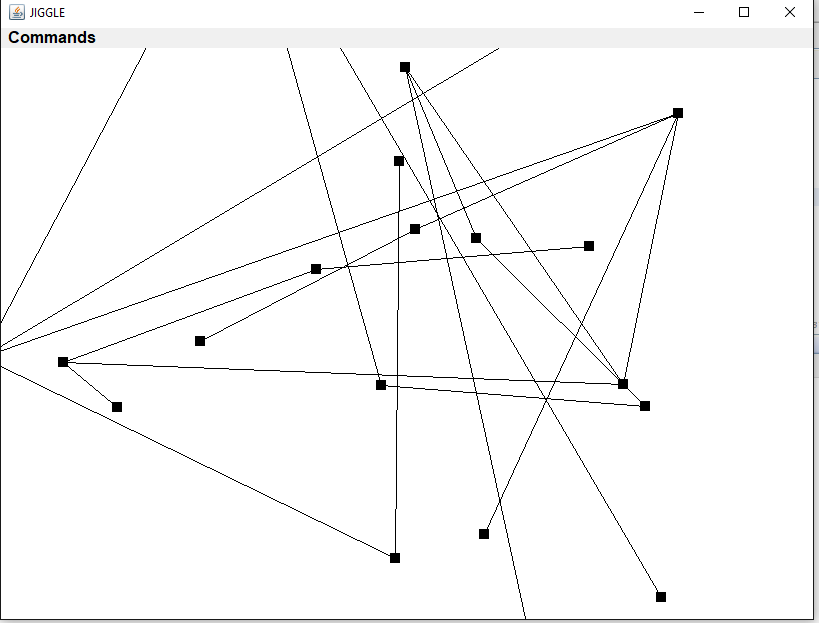
\includegraphics[width=7cm]{imagenes/jiggle_1.png}
		\label{subfig:jiggle_1}
	}
	\subfigure[Grafo luego de utilizar el algoritmo dirigido por fuerzas.]{
		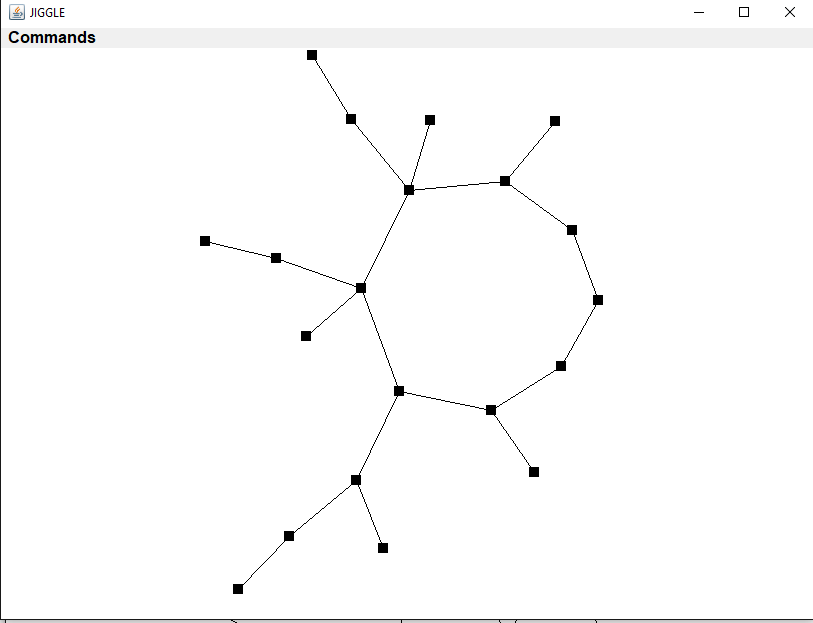
\includegraphics[width=7cm]{imagenes/jiggle_2.png}
		\label{subfig:jiggle_2}
	}
	\caption{Ejemplo de layout de grafo utilizando la herramienta Jiggle que provee Tunkelang para probar sus algoritmos.}
	\label{fig:jiggle}
\end{figure*}

% En el survey de Helen Gibson et al. \cite{gibson2013survey} se han recopilado gran variedad de algoritmos de layout, de los cuáles el más adecuado, con respecto a precisión y velocidad, para layout en modelado conceptual, es el algoritmo Dirigido por Fuerzas de Tunkelang \cite{tunkelang1998jiggle}. Este algoritmo  propone un modelo físico donde los nodos y arcos realizan fuerzas de repulsión entre ellos para evitar cruzamientos. Esta simulación se realiza por un tiempo dado hasta obtener el resultado deseado. En este la eficacia del resultado está ligada a las posiciones iniciales del grafo de entrada.

\section{Algoritmos Genéticos de Layout: TimGA y Hongmei He}
Los algoritmos de TimGA \cite{eloranta2001timga} utilizan grafos genéricos, es decir sin ninguna disposición particular de los nodos y arcos, para representar los individuos de sus algoritmos genéticos, como se muestra en la figura \ref{fig:timga_representacion}. En general este esquema de representación de individuos produce que las operación de variación que se tengan que definir sean mas complejas que con otras representaciones mas simples, y por lo tanto la computación del algoritmo se ve demorada.

Las pruebas realizadas sobre estos algoritmos han dado tiempos considerables para alcanzar un máximo local o global, debido a la gran variabilidad que existe entre grafos sin ningún estilo de dibujado particular \cite{gibson2013survey} (ver sección \ref{sec:estilos_de_dibujado}).

\begin{figure}[H]
	\centering
	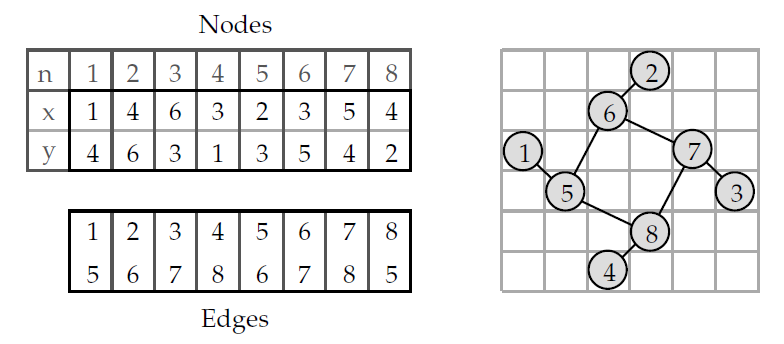
\includegraphics[width=13cm]{imagenes/timga_representacion.png}
	\caption{Representación de individuos en TimGA \cite{eloranta2001timga}.}
	\label{fig:timga_representacion}
\end{figure}

Por otro lado Hongmei He \cite{he2007parallelisation} utiliza para representar a sus individuos un estilo de dibujado de diagrama de arcos (ver sección \ref{sec:dibujado_diagrama_de_arcos}) y busca que la implementación del algoritmo permita utilizar paralelismo para agilizar su computación. A pesar de esto, los resultados que obtiene manejan tiempos considerables para la práctica debido en gran medida a que el grafo inicial del que parten para la generación de la población inicial es aleatorio y en ciertos casos puede llevar mucho tiempo alcanzar un máximo local \cite{gibson2013survey}.

Ambos algoritmos consideran como parámetro principal para evaluar el fitness de sus individuos el crossing number de estos (ver sección \ref{sec:crossing_number}).

% Por otro lado, otros algoritmos desarrollados para diagramas  genéricos que  utilizan métodos adaptativos, como por ejemplo algoritmos genéticos  \cite{eloranta2001timga, he2007parallelisation},  tienen problemas por la  considerable cantidad de generaciones que deben analizar, lo que conlleva a que  se consuma un tiempo elevado en alcanzar un máximo local o global. 
	
\section{Plugins de Layout para Protégé: OntoGraph, OWLViz y SOVA}
Protégé \cite{knublauch2004protege} incluye entre sus plugins pre-instalados, utilidades de visualización de ontologías como son OntoGraph \cite{falconer2010ontograf}[Fig. \ref{fig:ontograph}] y OWLViz \cite{horridge2010owlviz} [Fig. \ref{fig:owlviz}]. Estos brindan la capacidad a Protégé de visualizar una ontología en lenguaje OWL como un árbol, con conectores que simbolizan las relaciones de subsunción y las equivalencias entre las clases.

\begin{figure}[h]
	\centering
	\includegraphics[width=13cm]{imagenes/ontograph.png}
	\caption{Herramienta Protégé utilizando el plugin OntoGraph sobre una ontología en OWL.}
	\label{fig:ontograph}
\end{figure}

Los algoritmos de layout que disponen incluyen una distribución en forma de árbol descendiente o lateral. En el caso de OntoGraph también incluye un algoritmo de layout basado en un sistema de resortes (Spring Systems) \cite{kobourov2012spring}[Fig. \ref{fig:spring_systems}]. Este algoritmo funciona de manera similar al de dirigido por fuerzas de Tunkelang \cite{tunkelang1998jiggle}, computando fuerzas de atracción entre los nodos adyacentes y fuerzas de repulsión entre todos los pares de nodos.

\begin{figure}[H]
	\centering
	\includegraphics[width=13cm]{imagenes/spring_systems.png}
	\caption{Ilustración de un sistema de resortes genérico: empenzando desde posiciones aleatorias, trata al grafo como un sistema de resortes y busca encontrar una configuración estable \cite{gajer2002grip}.}
	\label{fig:spring_systems}
\end{figure}

\begin{figure}[h]
	\centering
	\includegraphics[width=10cm]{imagenes/owlviz.jpg}
	\caption{Herramienta Protégé utilizando el plugin OWLViz sobre una ontología en OWL.}
	\label{fig:owlviz}
\end{figure}

% Illustration of a generic spring embedder: starting from random positions, treat the graph as spring
% system and look for a stable configuration [32].

% This algorithm is similar to that of Eades in that both algorithms compute attractive forces
% between adjacent vertices and repulsive forces between all pairs of vertices

\section{OWLGrEd}
OWLGrEd \cite{liepinvs2014owlgred} es una herramienta de visualización de ontologías OWL, la cuál al momento de renderizar el diagrama utiliza algoritmos de layout. Los diagramas en OWLGrEd utilizan un layout Ortogonal \cite{bekos2012smooth}[Fig. \ref{fig:ortogonal}] sobre las relaciones, a excepción de las relaciones de herencia, las cuales las muestra con un layout jerárquico. Las relaciones de herencia fluyen desde un lado del diagrama hacia el lado opuesto, y las demás relaciones fluyen perpendicularmente a estas, como puede verse en la figura \ref{fig:owlgred}. Esto es debido a que las relaciones de herencia típicas de un diagrama OWL tienden a leerse mas fácilmente de izquierda a derecha y guían a un diagrama mas compacto.

\begin{figure}[h]
	\centering
	\includegraphics[width=13cm]{imagenes/owlgred.png}
	\caption{Visualización una ontología OWL en OWLGrEd \cite{liepinvs2014owlgred}.}
	\label{fig:owlgred}
\end{figure}

\begin{figure*}[h]
	\centering
	\subfigure[]{
		\includegraphics[width=5cm]{imagenes/ortogonal_1.png}
		\label{subfig:ortogonal_1}
	}
	\subfigure[]{
		\includegraphics[width=5cm]{imagenes/ortogonal_2.png}
		\label{subfig:ortogonal_2}
	}
	\caption{Ejemplo de un grafo visualizado con un layout ortogonal y con un estilo de diagrama de arcos \cite{bekos2012smooth}.}
	\label{fig:ortogonal}
\end{figure*}

% OWLGrEd diagrams use the orthogonal layout where the inheritance-defining
% relations (i.e. subclass-of relations between classes and instance-of relations
% between classes and instances) are presented in a hierarchical layout (i.e. they
% “flow” from one side of the diagram to the opposite side) and all other relations
% “flow” in the direction perpendicular to it. We have observed that for a typical
% OWL diagram the horizontal direction (left-to-right) seems to be the more
% readable and the one which leads to more compact diagrams.

\section{VOWL}
Los grafos son visualizados en VOWL \cite{lohmann2016visualizing}[Fig. \ref{fig:vowl}] utilizando el algoritmo de layout dirigido por fuerzas. Este layout tiene a ordenar los nodos de tal manera que las clases con mas conexiones este ubicadas mas próximas al centro de la visualización, y viceversa las que tienen menos conexiones mas próximas a la periferia. En este sentido, el layout dirigido por fuerzas ayuda a reflejar la importancia relativa de las clases en el grafo que está siendo visualizado, ya que el número de conexiones de una clase es usualmente un indicador de la importancia que esta tiene en la ontología \cite{peroni2008identifying}.

En VOWL algunos conceptos pueden aparecer multiplicados varias veces como nodos en la visualización del grafo. Esto ayuda a que el layout dirigido por fuerzas no tenga que ser forzado a resolver cruces de arcos complejos, por lo que relaja la visualización y facilita la navegabilidad. Para realizar tal multiplicación, VOWL sigue un conjunto de reglas que determinan que elementos pueden multiplicarse ya sea, para una clase en particular o para el grafo completo.

\begin{figure}[H]
	\centering
	\includegraphics[width=13cm]{imagenes/vowl.png}
	\caption{Interfaz de VOWL que permite visualizar una ontología y posee una barra de herramientas para configurar algunas preferencias. \cite{lohmann2016visualizing}.}
	\label{fig:vowl}
\end{figure}


% By default, VOWL graphs are visualized in
% a force-directed layout. Such a layout tends to arrange
% the nodes in a way that highly connected classes are
% placed more to the center of the visualization, whereas
% less connected ones are placed rather in the periphery.
% Thus, the force-directed layout helps to reflect the relative importance of the classes in the resulting graph
% visualization, as the number of connections of a class
% is often an indication of its importance in the ontology [84]. Moreover, graph layouts created with forcedirected algorithms are perceived to be aesthetically
% pleasant, since all edges have roughly the same length
% and since they tend to avoid edge crossings, which increases the readability of the visualization [5].
% In the same spirit as some elements are merged in
% VOWL, others are multiplied so that they may appear
% more than once in the graph. This helps to relax the
% energy of the force-directed layout and reduces the visual prominence of generic ontology concepts. Multiplication is based on the aforementioned splitting rules
% that determine whether there is no multiplication for
% elements, multiplication for each connected class, or
% multiplication across the entire graph. For instance,
% the generic class owl:Thing is multiplied in a way
% that it is added once for every class it is connected to,
% whereas datatype nodes appear once for every datatype
% property (cf. Figure 1).

% Algunas  herramientas para modelado ontológico tales como OWLViz \cite{horridge2010owlviz}, OntoGraph \cite{falconer2010OntoGraph}, SOVA \cite{kunowski2012sova}, OWLGrEd \cite{cerans2012advanced}, VOWL \cite{lohmann2014protegevowl} e ICOM \cite{fillottrani2012icom}, poseen algoritmos de layout automático, pero con ciertas limitaciones.  En primer lugar, OWLViz, OntoGraph y SOVA son plug-ins de Protégé \cite{knublauch2004protege} que utilizan grafos como lenguaje gráfico para ontologías. Por lo tanto, si bien ofrecen algoritmos visuales, están limitados en cuanto a la expresividad gráfica subyacente. ICOM y OWLGrEd están basados en los lenguajes de modelado conceptual EER y UML, respectivamente. Ambos permiten representar ontologías OWL \cite{hitzler2009owl} y poseen capacidades de layout automático. Sin embargo, solo proveen un conjunto de alineamientos fijos y estáticos. Además, el soporte gráfico de ICOM está actualmente descontinuado. Por último, VOWL también implementa una visualización dinámica pero, al igual que los plug-ins previos, usa grafos como modelos para OWL y no lenguajes de modelado conceptual.

\section{Análisis y Comparación}
El tipo de algoritmos de layout que utilizan OntoGraph, OWLViz, SOVA y OWLGrEd son útiles para grafos planares o de tipo árbol, por lo general para representaciones de ontologías OWL que presentan una jerarquía muy estricta entre sus elementos. Debido a esto, no consideran propiedades de dibujado como el crossing number u optimización de área, si no que se realizan teniendo en cuenta un criterio fijo y estático de organización, debido a que la forma de los grafos siempre será análoga.

En el caso particular de VOWL, este utiliza el algoritmo dirigido por fuerzas, pero nuevamente aprovecha el lenguaje de la representación a su favor, ya que para evitar problemas de cruzamientos multiplica los nodos que generan arcos que rompen la estructura de árbol jerárquica y los coloca en cada nodo como un hijo.

Estos algoritmos cuando queremos aplicarlos sobre modelos conceptuales comienzan a tener complicaciones, debido a la gran variedad de formas que puede tener un grafo para visualizar un diagrama en algún lenguaje de modelado conceptual. En este sentido, se buscaron otro tipo de técnicas mas generales para trabajar sobre layout de grafos, como son las de TimGA y Hongmei He, las cuales atacan el objetivo desde el problema de crossing number, pero sus resultados en la practica tienen complicaciones de eficiencia.

En conclusión, un punto medio entre estas técnicas es lo que se intenta resolver para alcanzar un algoritmo de layout mas óptimo para utilizar sobre diagramas de modelado conceptual.
\label{cap6}
\chapter{Conclusiones}
En esta Tesis se introdujeron el diseño y la implementación de un algoritmo para optimizar grafos completos y de uno genético, denominado {\sc ArcGen}, para mejorar grafos no completos. El objetivo de ambos es lograr un menor Crossing Number en grafos no dirigidos, mediante la utilización de la representación gráfica de Diagrama de Arcos.
	
Se describieron los detalles del desarrollo y se presentaron resultados experimentales que muestran una disminución en la cantidad de cruces entre el layout original y el mejor individuo obtenido después de aplicar el algoritmo.

%El objetivo de estos algoritmos es utilizar una estructura sencilla sobre la que se puedan plantear algoritmos de complejidad NP-completo buscando obtener un mínimo Crossing Number. 

El layout obtenido  a partir de {\sc ArcGen} no es el resultado final que visualizará el usuario en una herramienta gráfica de modelado, sino que se utiliza como entrada por otro algoritmo que traslada las posiciones de los nodos y arcos de manera que se pueda generar una visualización del mismo grafo pero de una manera más amigable al usuario. Este paso es la integración con el algoritmo de fuerzas de Tunkelang, la cuál permitió finalizar el ciclo del algoritmo de layout obteniendo una visualización final utilizable.

Para realizar las pruebas necesarias se implemento una herramienta que permitió visualizar los resultados de los algoritmos como diagramas de arcos y facilitar su depuración. En la misma se incluyen todos los algoritmos desarrollados y la integración con librerías externas para utilizar el algoritmo de fuerzas y permitir la visualización de grafos genéricos.

%Este último paso es la próxima etapa a desarrollar en este proyecto, para el cuál se tendrá en cuenta el lenguaje gráfico con el que se diseña el modelo y los criterios para los diferentes constructores de tales lenguajes. Los resultados obtenidos de los algoritmos implementados, se  consideran prometedores para la continuación del proyecto.

 \section{Trabajos Futuros}

Entre los trabajos futuros,  se encuentran la evaluación de  {\sc ArcGen} sobre modelos conceptuales reales y el cálculo de la complejidad computacional temporal de los algoritmos para alcanzar un mayor nivel de detalle en los resultados.

Por otro lado la integración de {\sc ArcGen} con otros algoritmos de visualización general, además del de fuerzas que fue utilizado, para evaluar si existe mejoría y un mejor resultado final. Como también el desarrollo de algoritmos específicos para cada tipo de lenguaje de modelado (UML, ER, ORM, etc) que permitan mapear los diagramas de entrada en un grafo preferente para su utilización en los algoritmos desarrollados y luego mapearlos nuevamente al lenguaje de modelado específico.

Finalmente, el desarrollo de una interfaz para integrar el algoritmo con herramientas de modelado como \emph{Crowd}. Formalizando un lenguaje para importar y exportar los diagramas con la herramienta. O bien, la integración de los algoritmos dentro de una herramienta específica para lograr una interacción mas rápida del usuario con los algoritmos de layout.

\vfill
\pagebreak
\addcontentsline{toc}{chapter}{Bibliografía}
\bibliographystyle{plain}

\bibliography{bibliography}






\end{document}
